\chapter{Tune for the Underlying Event}
\label{chap:OurTunefortheUnderlyingEvent}

This section focuses on the work in order to reproduce a similar tune to CP5 for the underlying event and minimum bias observables. This is done to test the ability of \textsc{mcnntunes} of being a valid tool for the tuning of Monte Carlo generators with real data. 
\\
In order to validate \textsc{mcnntunes} is has been decided to first perform a simpler tune with only two free parameters and then try to reproduce CP5 \cite{CPtunes} with all the five parameters variation.


\section{Introduction}

A different tune has been performed for the underlying event and minimum bias observables using the same distributions, listed in \chapRef{sec:Thedistributionsused} and used in CP5 tune, so we expect to get a similar result from the tune using  \textsc{mcnntunes}.
\\
Here is reported a quick reminder for the \textsc{pythia8} settings used in CP5 and in \textsc{mcnntune} tunes:
\begin{itemize}
	\item The NNLO PDF set used is \textsc{nnpdf}3.1 \cite{NNPDF:2017mvq}; 
	\item an $\alpha_s$ value equal for all the processes set to $0.118$ and running with a NLO evolution.
	\item The ISR is also ordered according to rapidity.
\end{itemize}
In the tuning procedure we employed both the \textsc{mcnntunes} operation modes described in the previous chapter: PerBin and Inverse models.

\section{First test: only two parameters variation}

The first simplified test we perform is the tuning varying only two parameters. The parameter chosen are the \texttt{Multiparton}\-\texttt{Interactions:}\-\texttt{pT0Ref} and 
\texttt{Multiparton}\-\texttt{Interactions:}\-\texttt{ecmPow}. These two parameters have been introduced in \secRef{sec:BasicConcepts}.
\\
The aim of this simplified test is to check the correct operation of \textsc{mcnntunes}  in a restricted parameters space.% it is simpler to learn the generator behavior and predict the corrects best values for the parameters. 
\\
\tableRef{table:variation_2params} shows the parameters space used in this first case. The other parameters are set to the CP5 values (also these are reported in the table as a reminder).

\begin{table}[!htb]
\centering
\begin{tabular}{l | c }
Parameter Name & Value \\ 
\hline \hline
\\[-0.85em]
	\texttt{MultipartonInteractions:pT0Ref} [$\mathrm{GeV}$] & $[1.0 - 3.0]$\\
	\texttt{MultipartonInteractions:ecmPow} & $[0.0 - 0.3]$\\
	\texttt{MultipartonInteractions:coreRadius} & $0.7634$\\
	\texttt{MultipartonInteractions:coreFraction} & $0.63$\\
	\texttt{ColorReconnection:range} & $5.176$
\end{tabular}
\caption{Parameters space for the two parameters test. The other parameters are set to the CP5 default values.}
\label{table:variation_2params}
\end{table}

\noindent During this first part we don't use the two distributions related to the single diffractive and non single diffractive event selection for a bug on the routine of the analyses that has been fixed up before the real tune.  
\\
Let now discuss the results obtained for the test with the two models.

\subsection{Per Bin Model results}

The result we obtain for the PerBin model are reported in \tableRef{table:resultPerBin_2param}. The PerBin model estimation of the best parameters is performed by a loss function minimization. The output of the minimizer is reported in \figRef{fig:resultPerBin_2param}, the loss function ($\chi^2/\mathrm{dof}$) is the orange one, while the best parameter is marked by a solid red line.


\begin{figure}[!htb]
	\centering
	\noindent
	\begin{subfigure}{.45\textwidth}
		\centering
		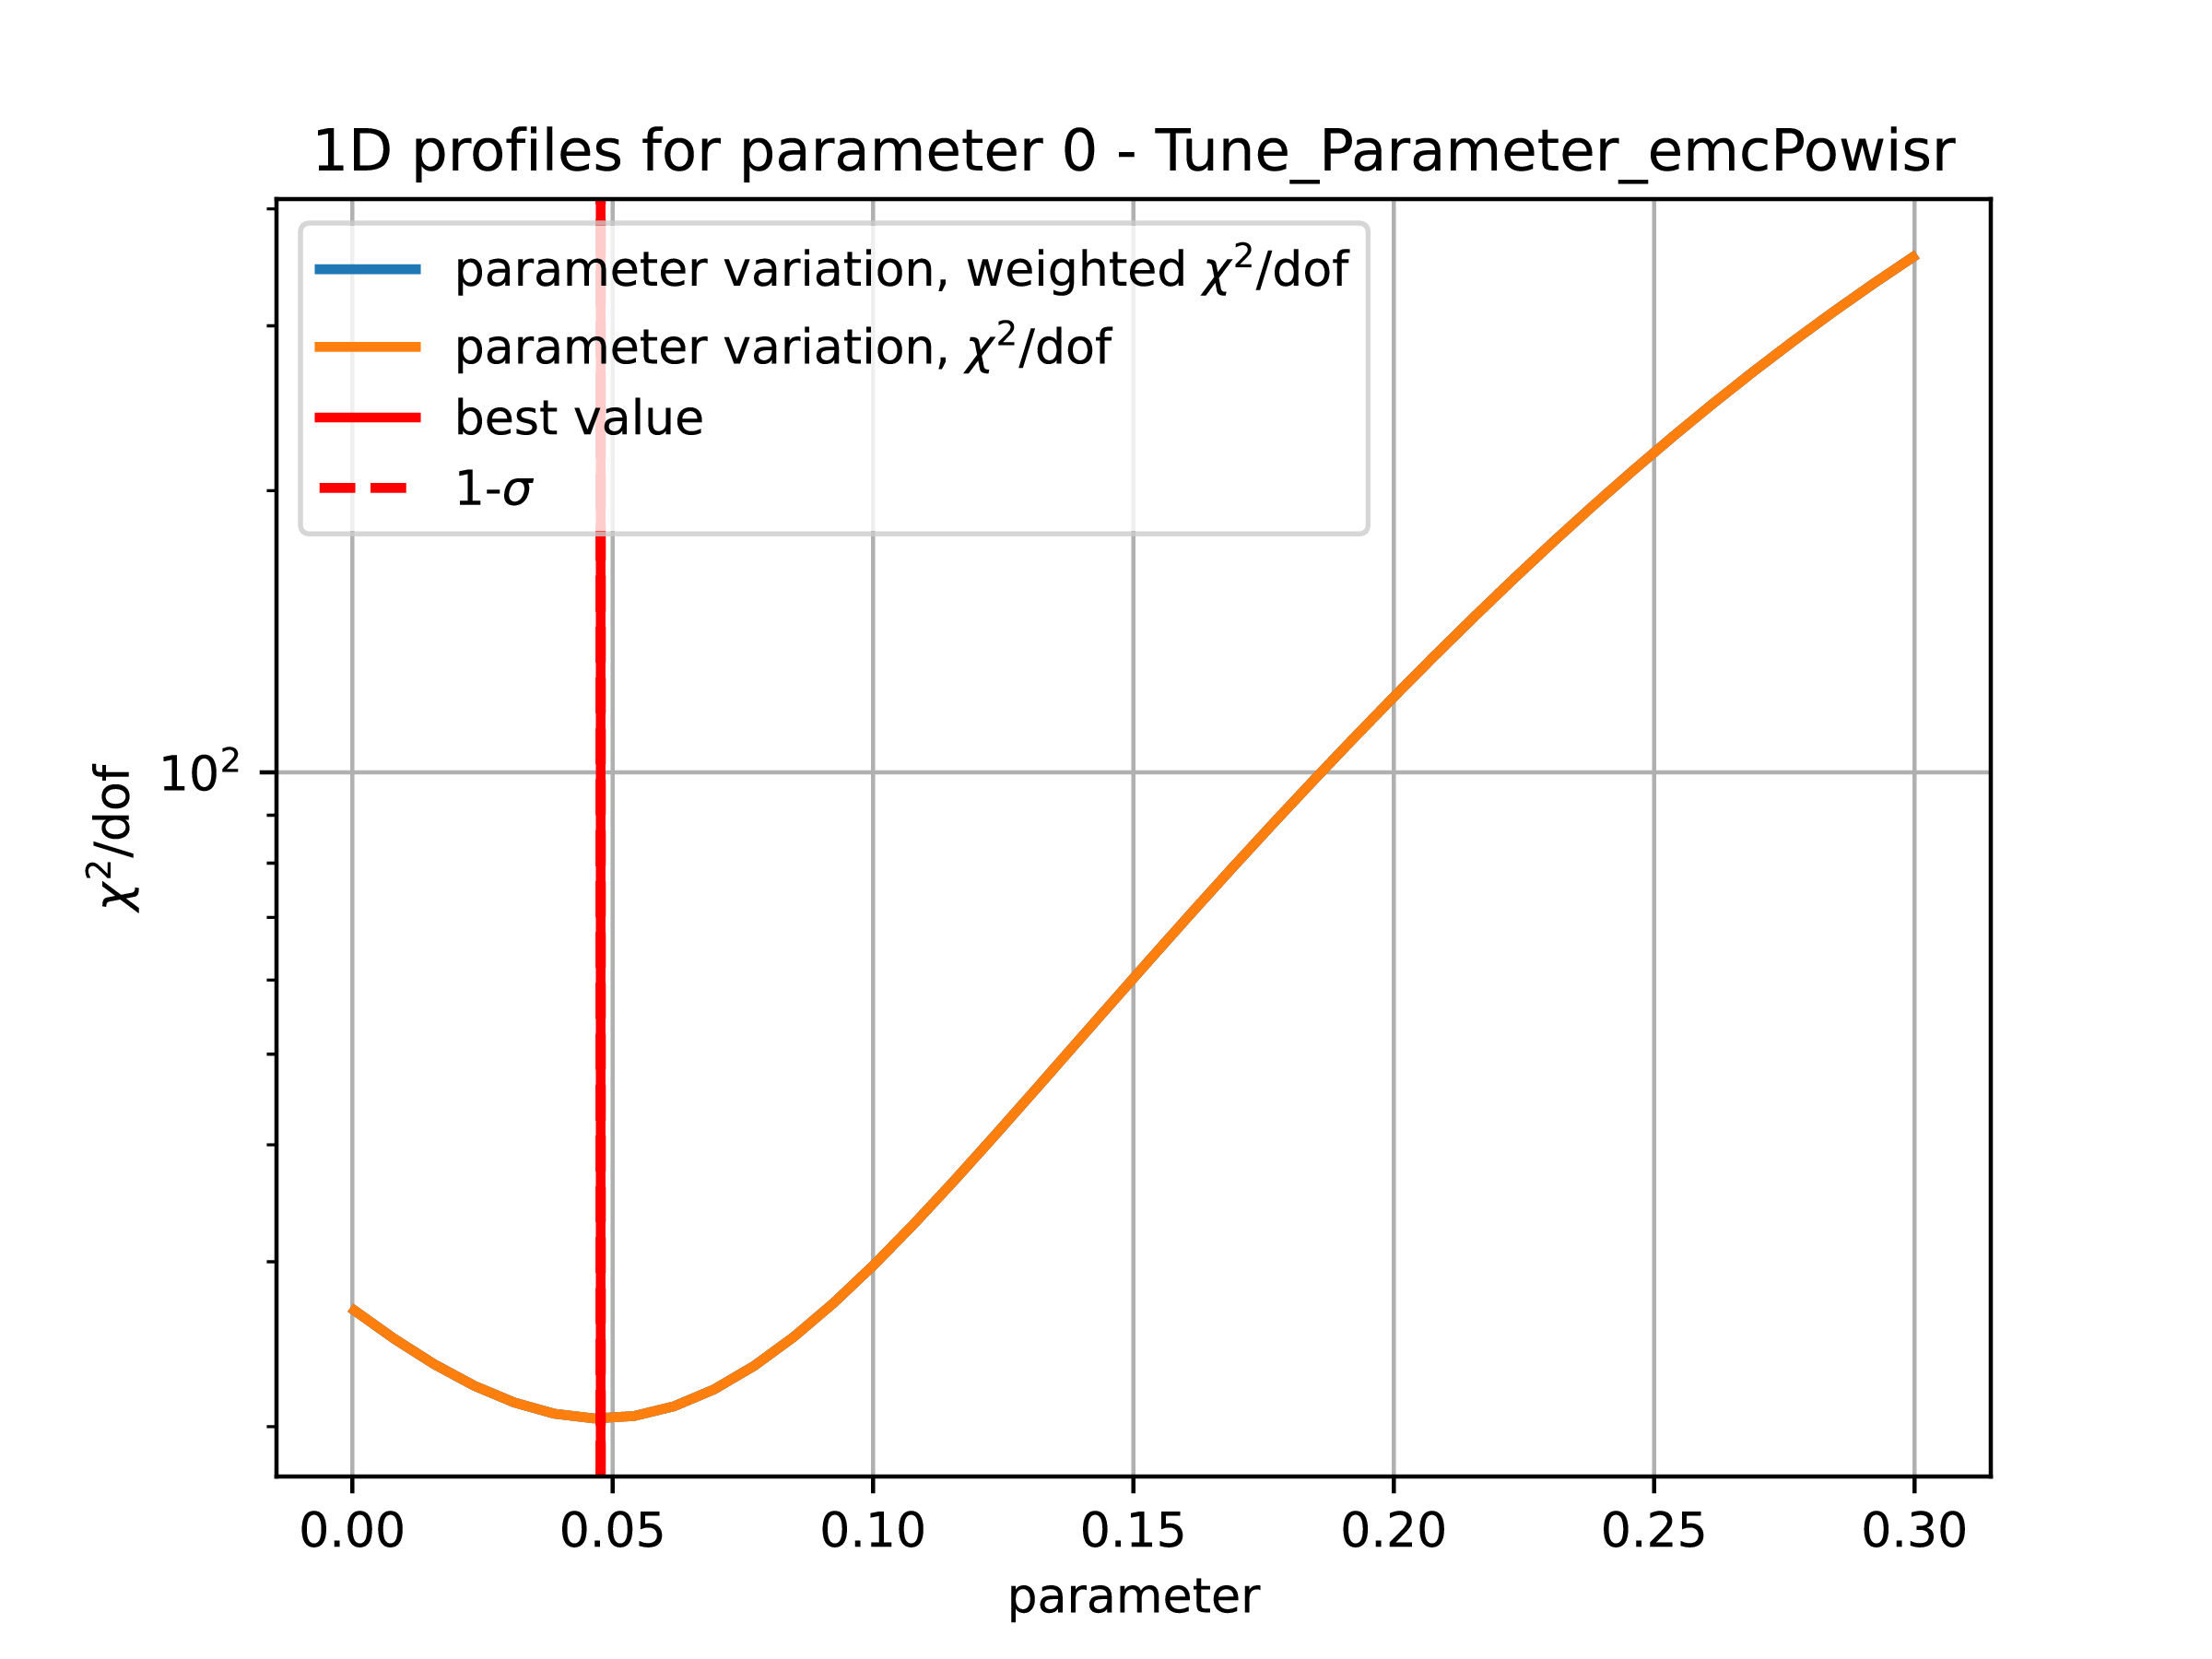
\includegraphics[width=\textwidth]{{img/Plots_2params_Finale/chi2_0.jpg}}
	\end{subfigure}%
	\begin{subfigure}{.45\textwidth}
		\centering
		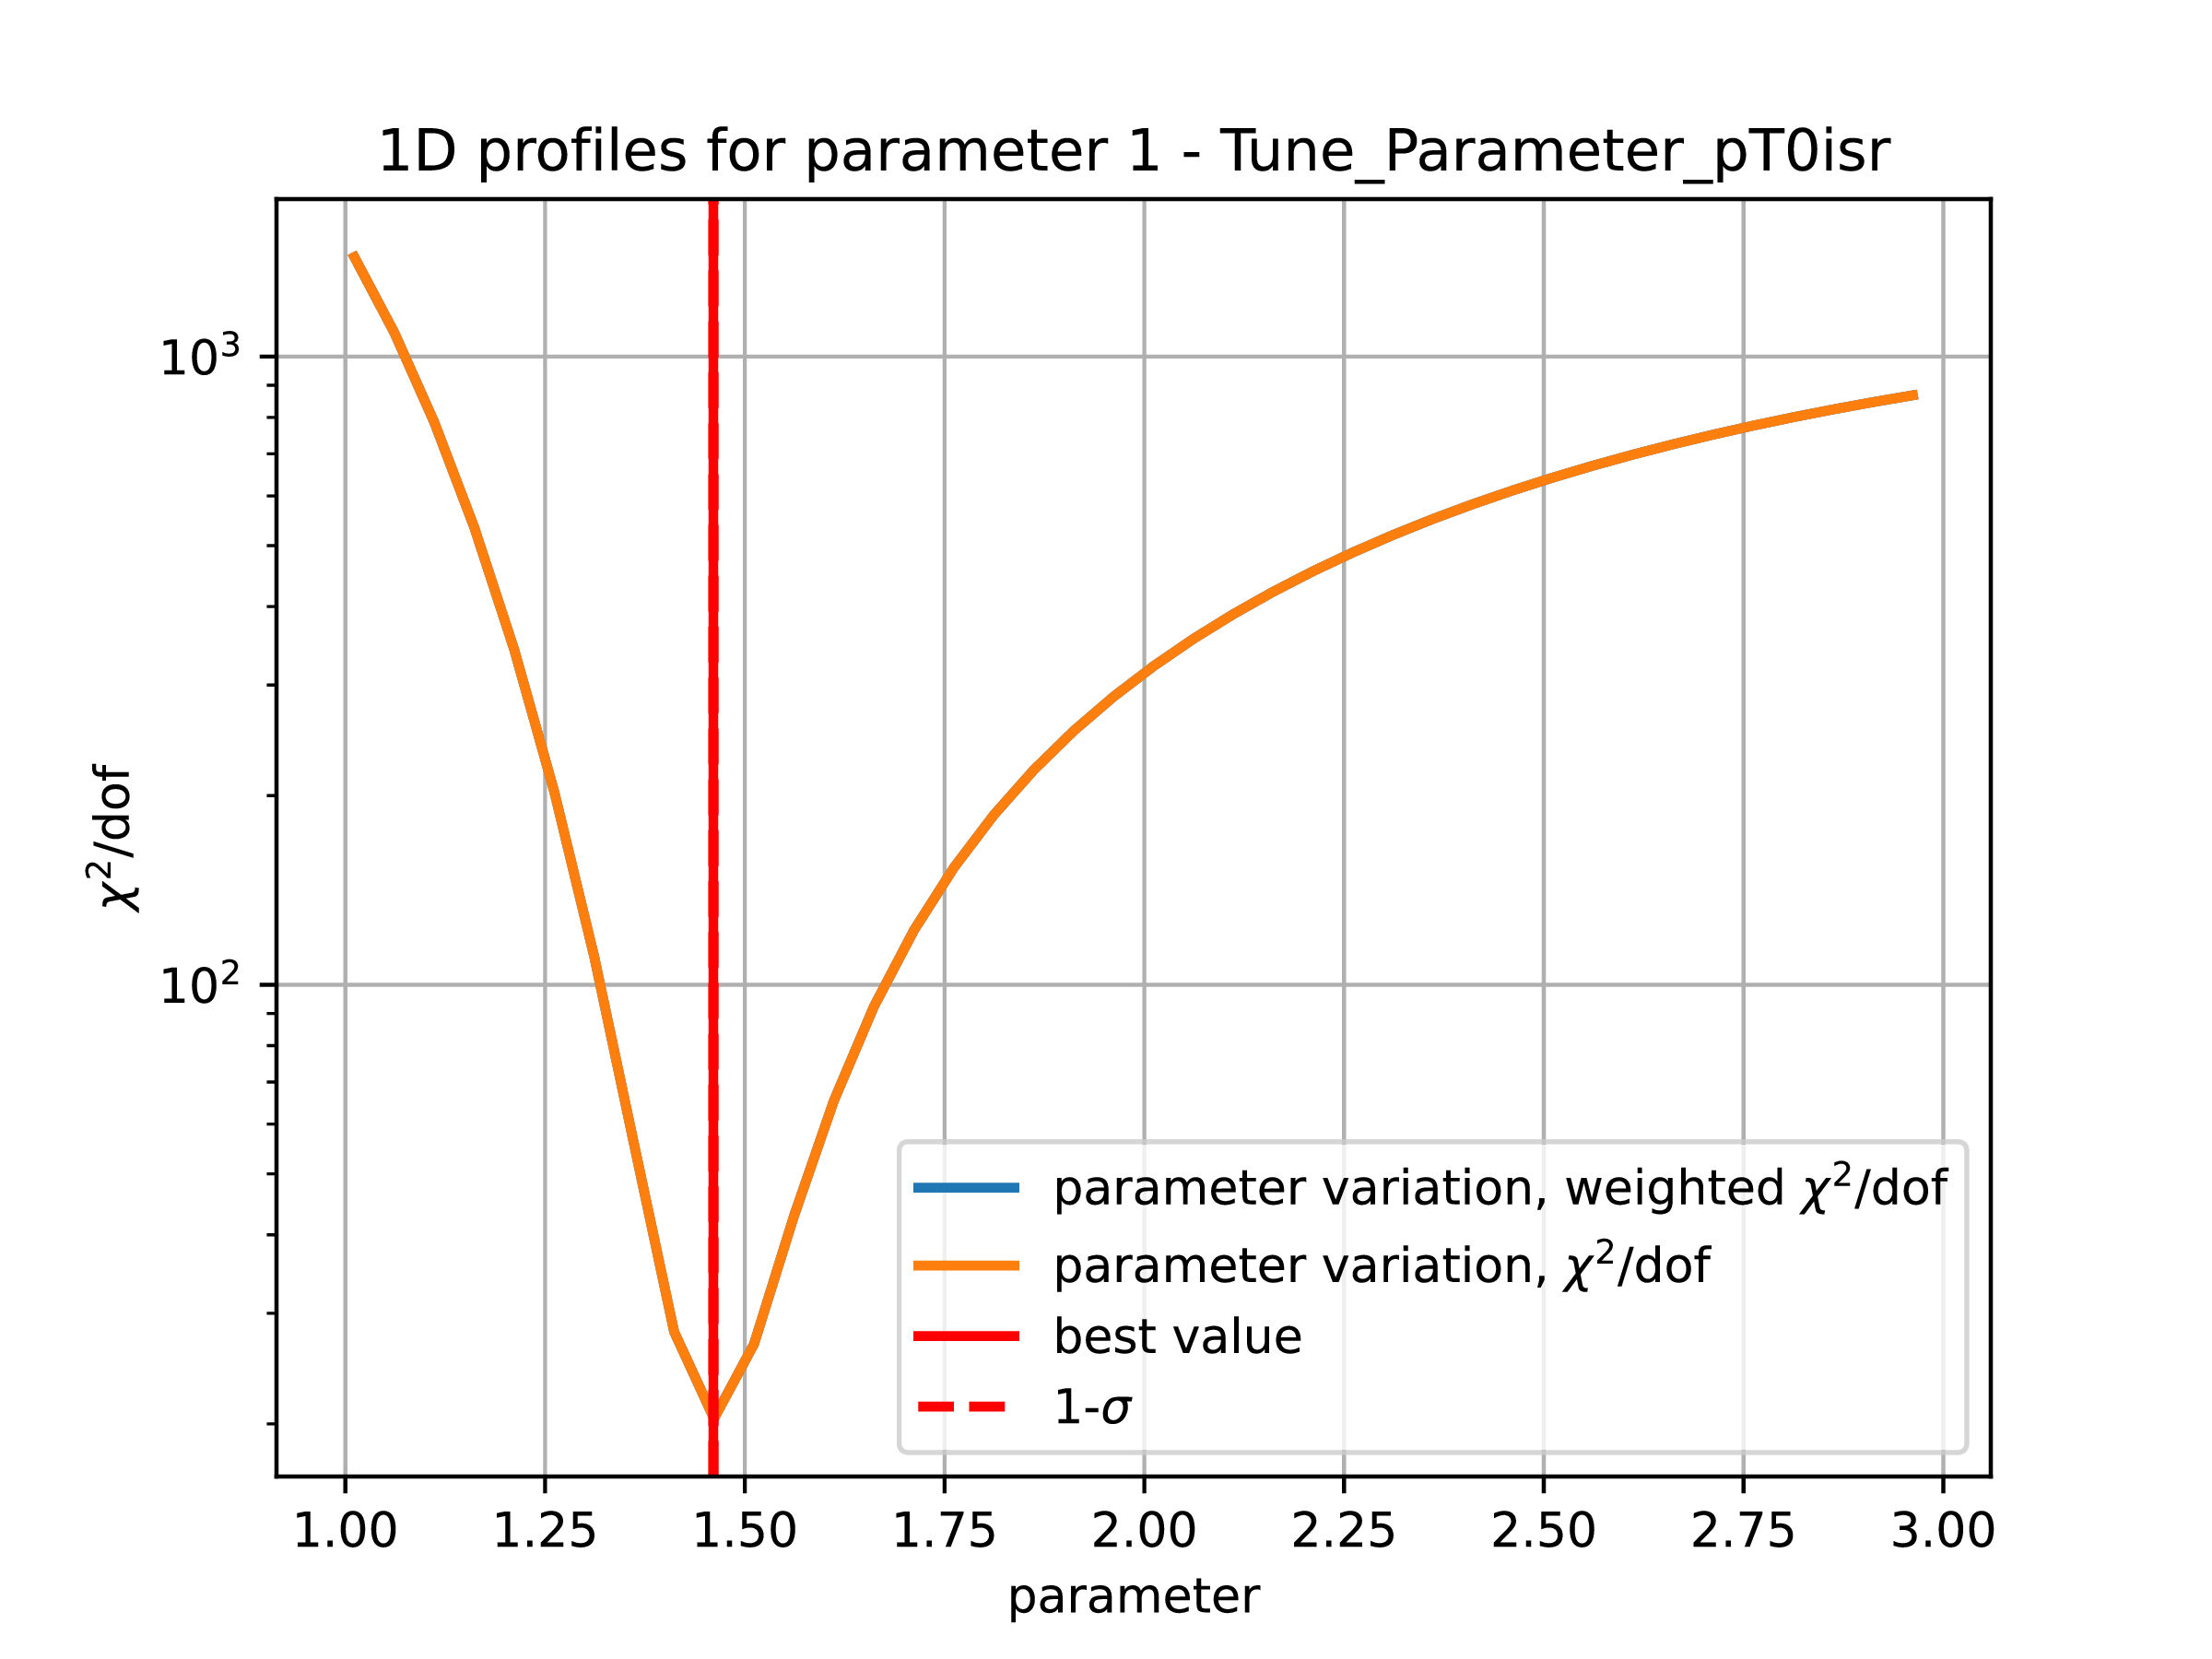
\includegraphics[width=\textwidth]{{img/Plots_2params_Finale/chi2_1.jpg}}
	\end{subfigure}
	\caption{The figure shows the output of the minimizer for each parameter. The right one refers to the \texttt{MPI:ecmPow} while the left one to the \texttt{MPI:pT0Ref}. The orange line is the $\chi^2/DoF$ as a function of the parameter values, the solid red line indicated the best estimation for the parameters.}
	\label{fig:resultPerBin_2param}
\end{figure}

\noindent The estimated parameters for the tune are also reported in \tableRef{table:ResultInverse_2params} with a comparison on CP5 boundary for each parameter. The errors on the parameter estimated with PerBin model are not reported here because a correct error implementation, as the one described in \secRef{sec:PerBinModel}, was not yet implemented in the software at the moment of this test, but here we can see an example of the old error estimation. The errors estimated with the old method are too small to represent a credible interval, in fact the errors lines (dashed red lines) are overlapped to the line of the parameter estimation in both the figures. The predicted errors were 3 or 4 orders of magnitude smaller than the parameter values. 
\\
As we expected the results we get are similar to the ones obtained from the CP5 tune. The distributions obtained from the simulation using this parameters are shown below (\secRef{subsec:Overall2PARAMS}) together with results from Inverse model and CP5.

%\begin{table}[!htb]
%\centering
%	\begin{tabular}{l | c | c}
%		Parameter & Value & CP5 (down \& up) \\ \hline\hline
%		\\[-0.85em]		
%		\texttt{MultipartonInteractions:pT0Ref} & $ 1.46064$ & $1.41-1.46$\\
%		\texttt{MultipartonInteractions:ecmPow} & $ 0.04771$ & $0.03$\\
%	\end{tabular}
%	\caption{Results for the PerBin model in two parameter variation test. The error evaluation was not correctly implemented yet and so the PerBin errors omitted in this table. The upper and lower limit for CP5 are also reported here for a direct comparison between the two tunes.}
%	\label{table:resultPerBin_2param}
%\end{table}

\medskip

An important observation is that our model is more sensible to some parameter respect to others.
\\
As an example, in \figRef{fig:param_vs_distributions} it is clear that our model is more sensible to the parameter \texttt{MultipartonInteractions:pT0Ref} (top) respect to 
\texttt{MultipartonInteractions:}\-\texttt{ecmPow} (bottom). This is reflected in the output of the minimizer, in which a larger sensitivity corresponds to a better defined minimum and vice versa. The top two panels show what happens when the distribution are very sensitive to the variation of the parameter as we can see on the left side the variation of the \texttt{pT0Ref} parameter leads to very different scenarios. This is reflected by the minimizer out in a well defined minimum and a smaller error on the parameter determination. A different scenario is displayed on the bottom panels of \figRef{fig:param_vs_distributions} where the distribution is less sensitive to the variation of the parameter \texttt{ecmPow} and so the minimum is less defined and so we are going to have a larger error on the estimation.

 
\begin{figure}[!htb]
\centering
\noindent
	\begin{subfigure}{.4\textwidth}
		\centering
		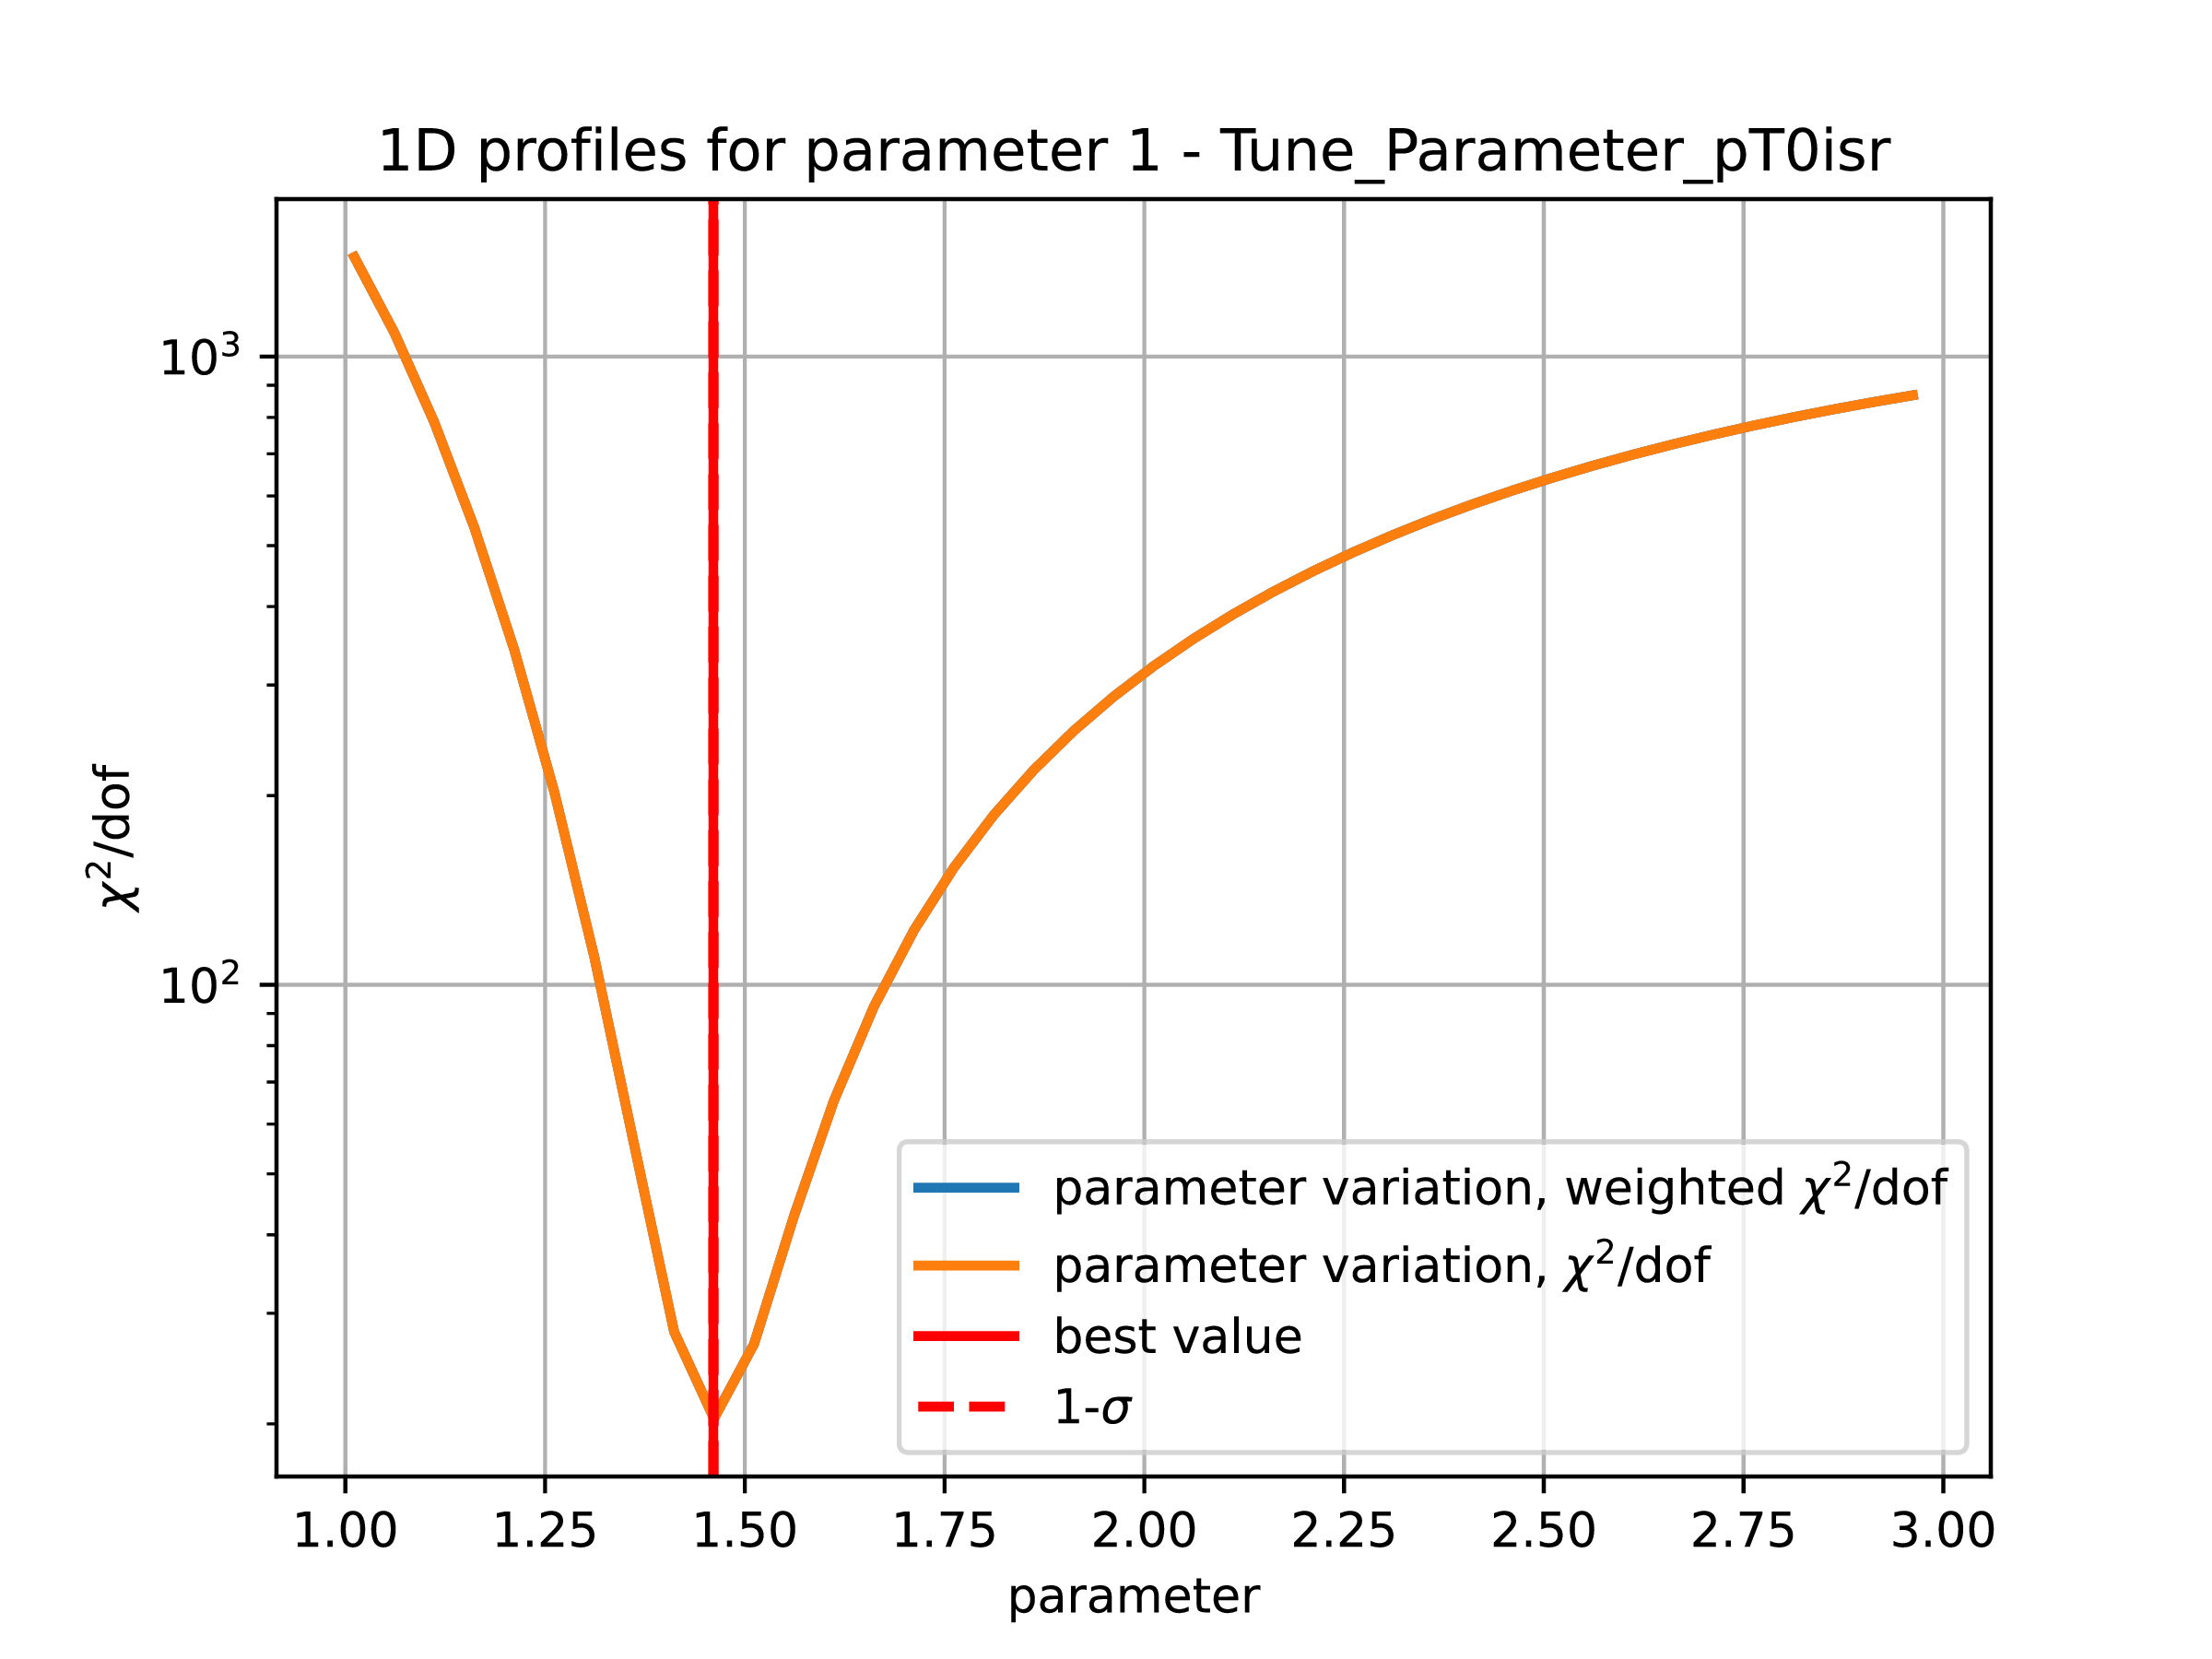
\includegraphics[width=\textwidth]{{img/Plots_2params_Finale/chi2_1.jpg}}
	\end{subfigure}%
	\begin{subfigure}{.07\textwidth}
		\centering
		\hspace{-4pt}
\includegraphics[width=\textwidth]{{img/blueRightarrow.pdf}}
	\end{subfigure}%
	\begin{subfigure}{.4\textwidth}
		\centering
		\includegraphics[width=\textwidth]{{img/Plots_pTzero/CMS_2015_PAS_FSQ_15_007/d01-x01-y01.pdf}}
	\end{subfigure}\\
\centering
	\begin{subfigure}{.4\textwidth}
		\centering
		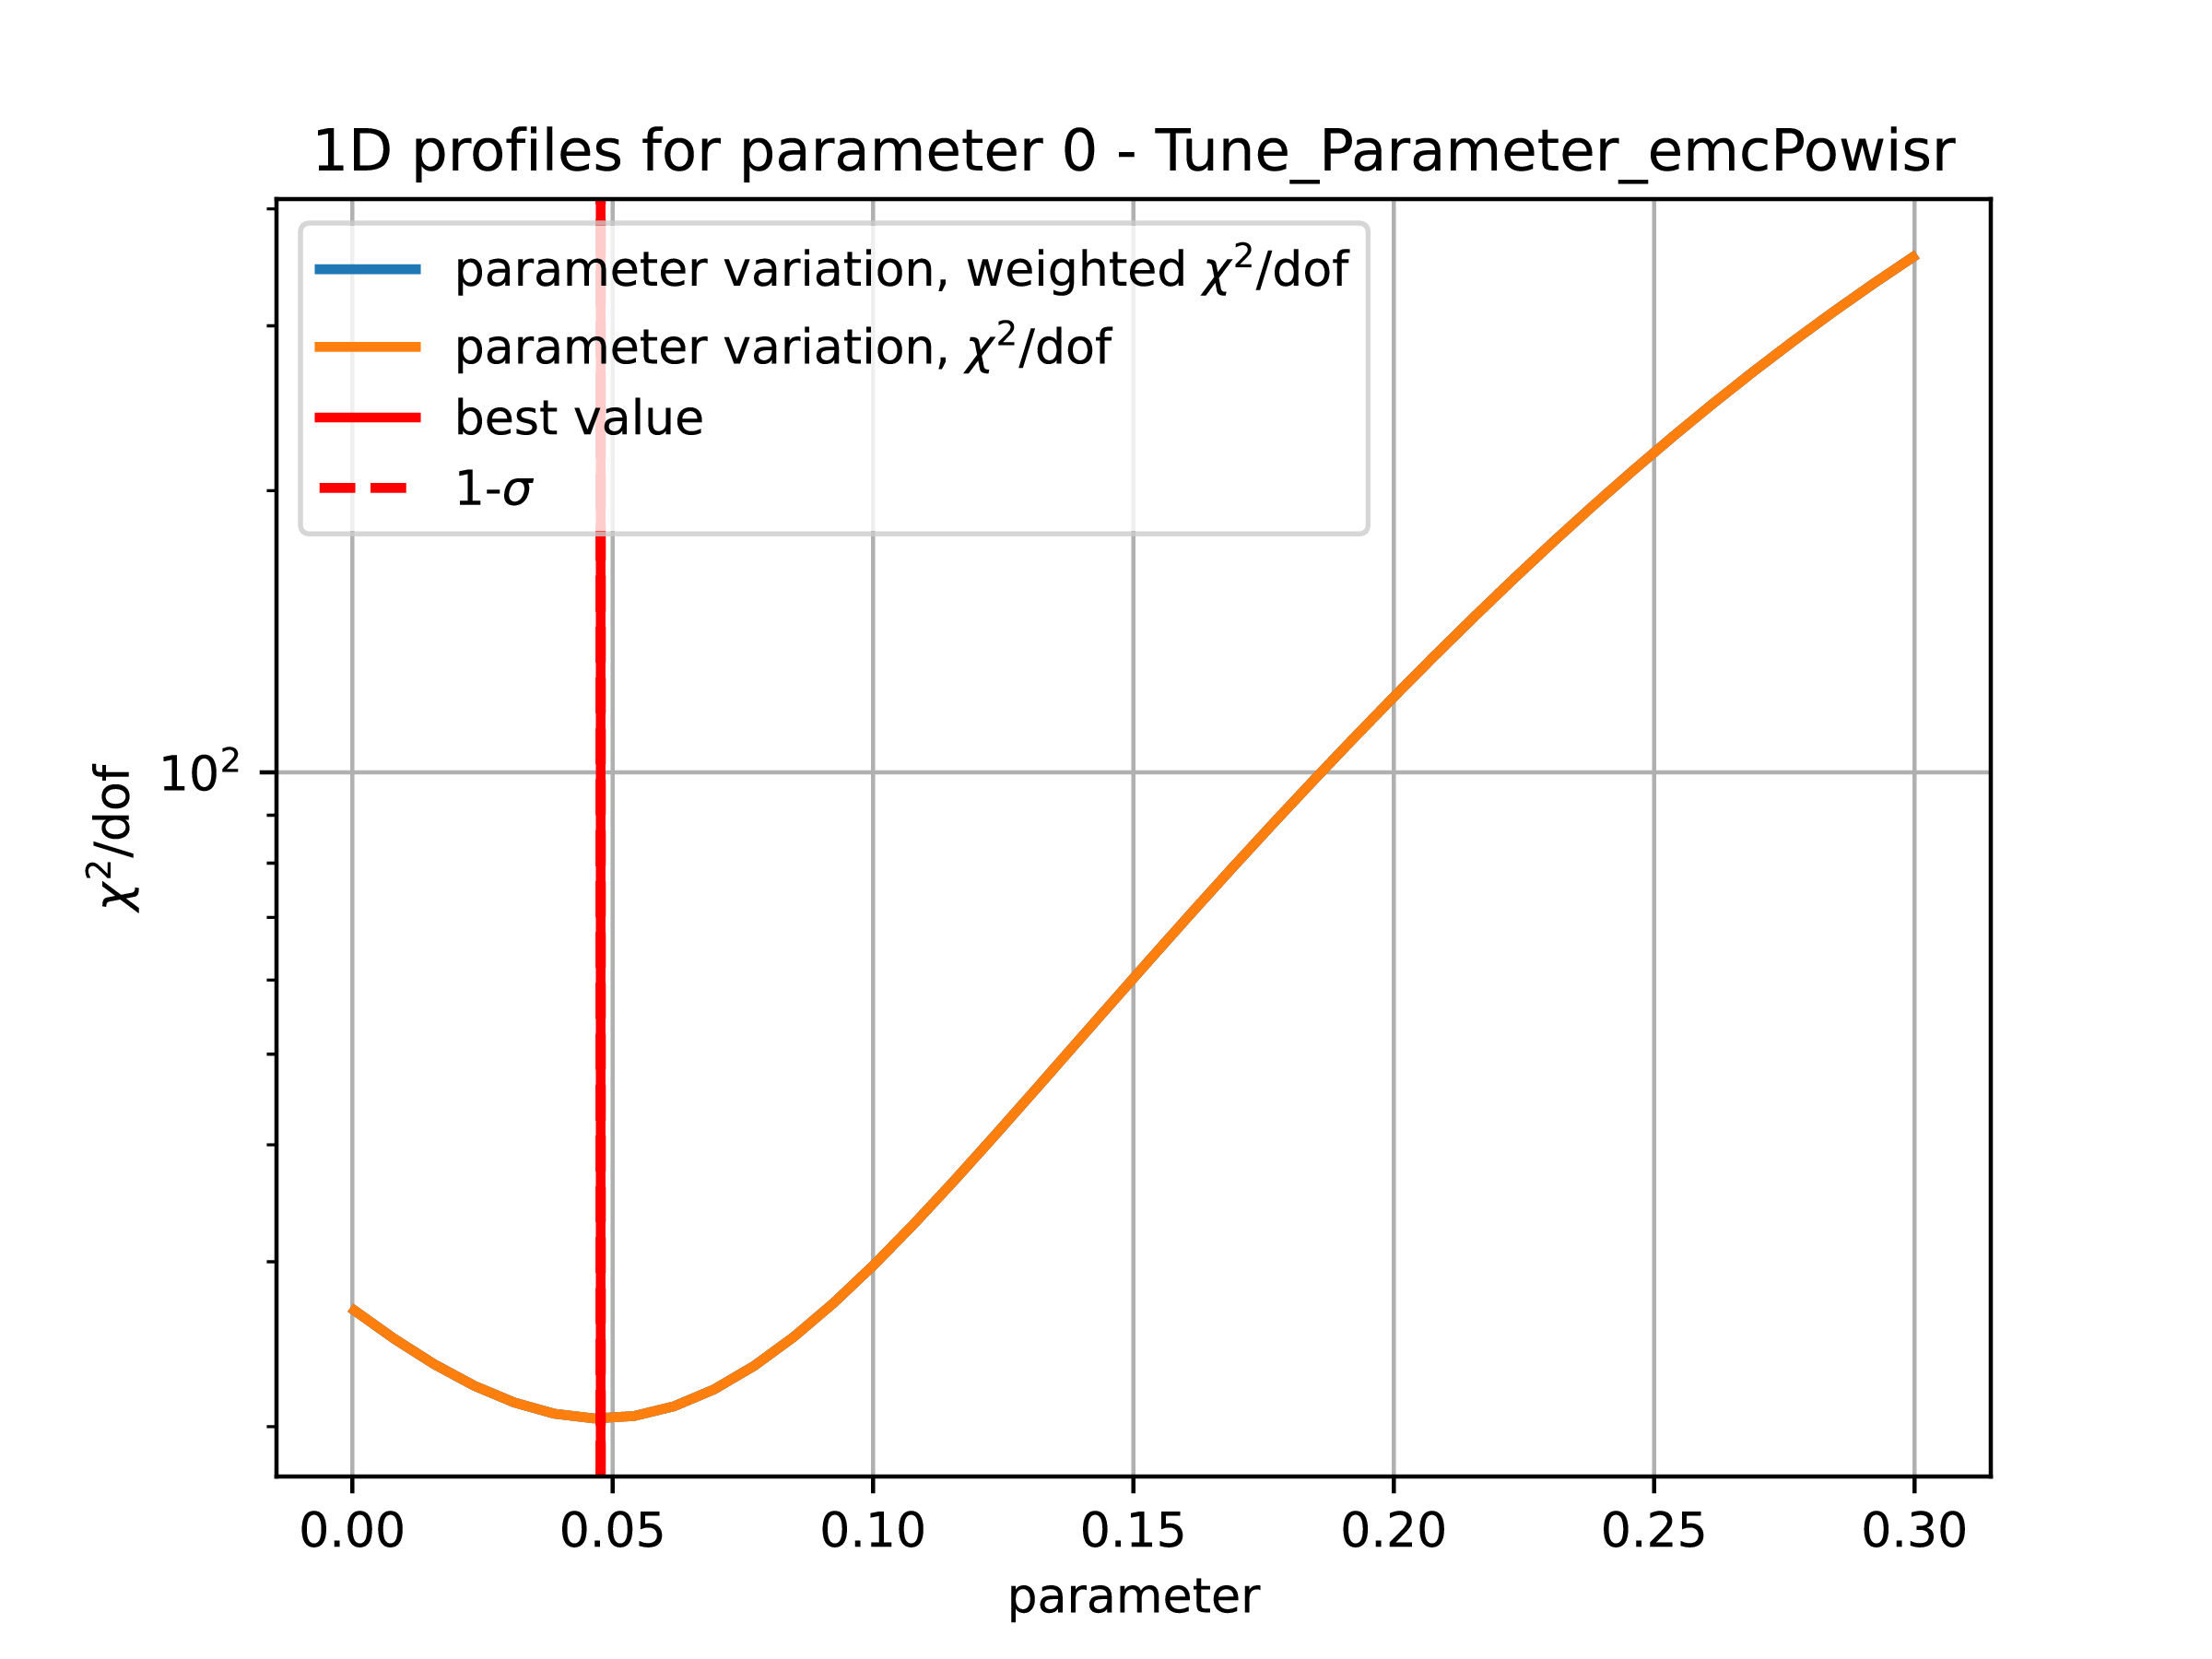
\includegraphics[width=\textwidth]{{img/Plots_2params_Finale/chi2_0.jpg}}
	\end{subfigure}%
	\begin{subfigure}{.07\textwidth}
		\centering
		\hspace{-4pt}
\includegraphics[width=\textwidth]{{img/blueRightarrow.pdf}}
	\end{subfigure}%
	\begin{subfigure}{.4\textwidth}
		\centering
		\includegraphics[width=\textwidth]{{img/Plots_ecmPow/CMS_2015_PAS_FSQ_15_007/d01-x01-y01.pdf}}
	\end{subfigure}
	\caption{the sensibility of the tuned distributions respect to the variation of the parameters related to the output of the minimizer. The top panels are related to \texttt{pT0Ref} while the bottom ones to \texttt{ecmPow}. The different colored lines in the 2 distributions (on the right) are the simulations with different values for the parameter. The black points are the data. }
	\label{fig:param_vs_distributions}
\end{figure}

\clearpage
\subsection{Inverse Model results}

The other operation mode offered by \textsc{mcnntunes} is the Inverse model. 
The results we get from the first test of the Inverse model are described here while the overall distribution are reported in next section together the ones from the PerBin Model. 
\\
As mentioned before to make this model work properly a hyperparameter optimization is necessary. The hyperparameter optimization used here was a scan of the architecture parameters shown in \tableRef{table:hyperpar_MinBias_2par}, where the number of trials (combinations of these parameters) was $1000$. In this case the best model we found is the one reported in \tableRef{table:hyperpar_2parTEST}.
\begin{table}[!htb]
	\centering
	\begin{tabular}{| l | c |}
	\hline
	Hyperparameter & Variation Range\\[2pt]\hline
	Number of hidden layer & 2-5 \\[2pt]
	Units per layer & 2-20 \\[2pt]
	Activation function & tanh, relu, sigmoid \\[2pt]
	Optimizer & {\small sgd, rmsprop, adagrad, adadelta, adam, adamax, nadam}\\[2pt]
	Epochs & 250-15000 in discrete steps\\[2pt]
	Batch size & 64-5000 in discrete steps\\[2pt] \hline
	Number of trials & 1000\\[2pt]\hline
	\end{tabular}
	\caption{Hyperparameter space scanned for the optimization of the NN architecture.}
	\label{table:hyperpar_MinBias_2par}
\end{table}


\begin{table}[!htb]
	\centering
	\begin{tabular}{ l | c }
	Hyperparameter & Value\\[2pt]\hline\hline
	Number of hidden layer & 4 \\[2pt]
	Units layers & [2,\,14,\,9,\,18] \\[2pt]
	Activation function & tanh \\[2pt]
	Optimizer & nadam\\[2pt]
	Epochs & 1000\\[2pt]
	Batch size & 500\\[2pt]
	\end{tabular}
	\caption{Best hyperparameters model found for the test with 2 parameters variation. The "Units layers" row indicates the number of units in each layer.}
	\label{table:hyperpar_2parTEST}
\end{table}

\noindent Once the best model is trained the output we get from this model is the distribution of predictions obtained by the resampling phase of the experimental data then fed to the network. The prediction spread for the two parameters test is shown in \figRef{fig:ResultInverse_2params} these are obtained from the re-sampling phase using the multivariate Gaussian distribution described in \eqRef{eq:gaussianDristribution}. 

\begin{figure}[!htb]
	\centering
	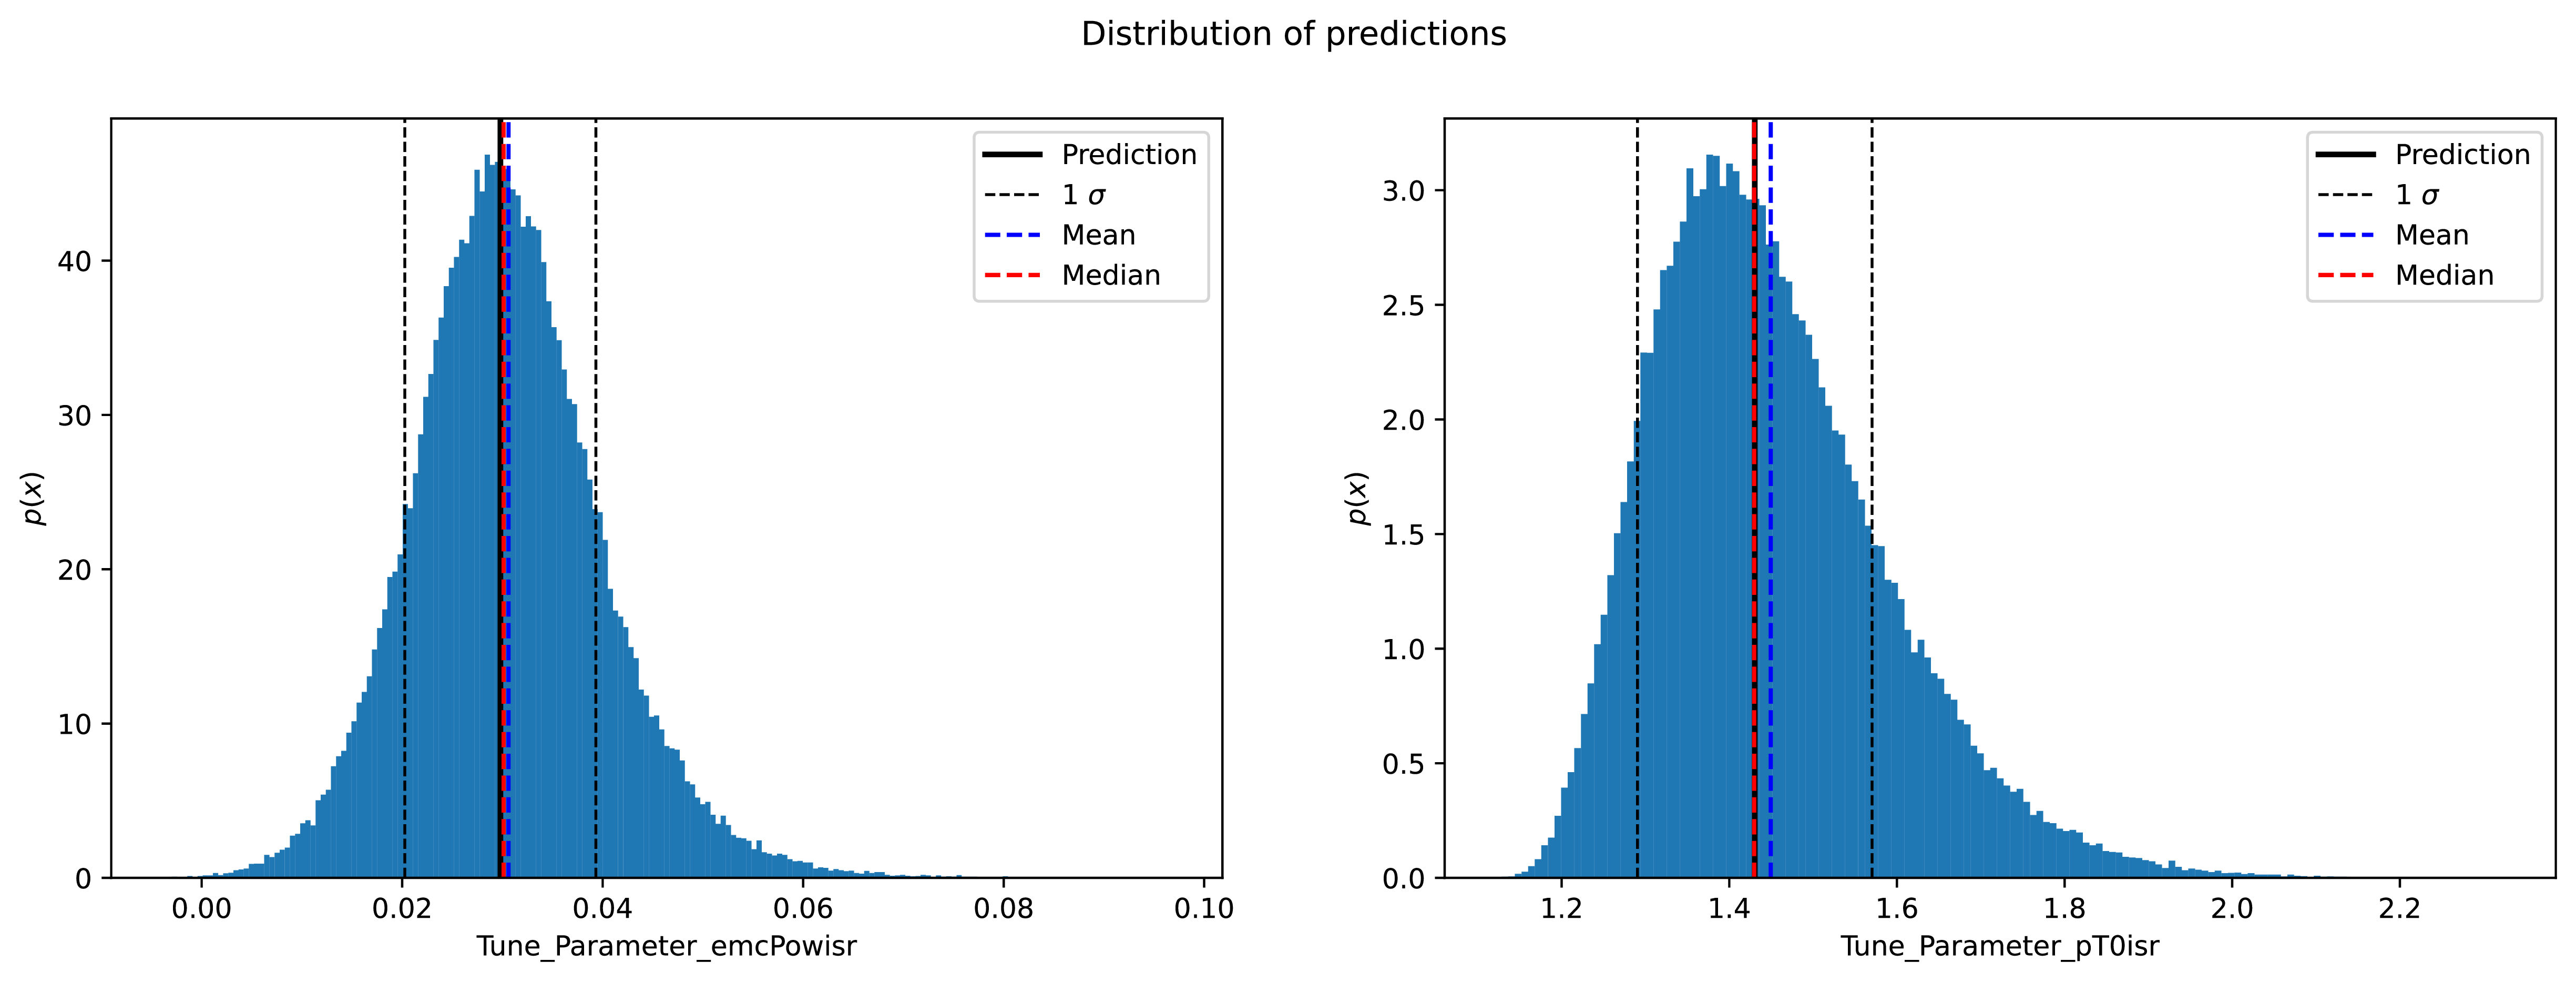
\includegraphics[width=0.9\textwidth]{{img/Plots_2params_Finale/2params_prediction_spread.jpg}}
	\caption{The spread of predictions we get as output from the Inverse Model. the right one refers to the \texttt{ecmPow} parameter and the left one to \texttt{pT0Ref}. The parameters predicted are marked by the solid black line while the error is evaluated using the standard deviation indicated by the dashed black lines.}
	\label{fig:ResultInverse_2params}
\end{figure}

\noindent The estimated parameter are marked by the solid black line, while the dotted black lines are the error on the parameter.
The value we get from the tune are also reported in \tableRef{table:ResultInverse_2params} together with the CP5 values.
In this case the error estimation is correctly implemented and a direct comparison between the value is possible. Looking at the values reported in the table it is clear that the two tune are compatible. 



%\begin{table}[!htb]
%\centering
%	\begin{tabular}{l | c | c}
%		Parameter & PerBin & Inverse & CP5 (down \& up)\\ \hline\hline
%		\\[-0.85em]		
%		\texttt{MPI:pT0Ref} & $ 1.46064$ & $ 1.43 \pm 0.14 $ & $1.41 - 1.46$ \\[2pt]
%		\texttt{MPI:ecmPow} & $ 0.04771$ & $ 0.0298 \pm 0.0095 $ & $0.03$\\[2pt]
%	\end{tabular}
%	\caption{Results for the PerBin and Inverse models in two parameter variation test. The upper and lower limit for CP5 are also reported here for a direct comparison between the two tunes.
%The two predicted parameters for the Inverse model are compatible to the one in CP5. While a direct comparison is not possible for the PerBin model, due to the not properly evaluated error, but the parameters are quite similar to the expected ones.}
%	\label{table:ResultInverse_2params}
%\end{table}


\clearpage
\subsection{Overall results}
\label{subsec:Overall2PARAMS}

In this section we are going to show some overall results for the first test with only two free parameters. We are not going to show all the graphs here, we list them all in the  \refApp{appendix:test}.

\begin{table}[!htb]
\centering
	\begin{tabular}{l | c | c}
		Parameter & PerBin & Inverse & CP5 (down \& up)\\ \hline\hline
		\\[-0.85em]		
		\texttt{MPI:pT0Ref} & $ 1.46064$ & $ 1.43 \pm 0.14 $ & $1.41 - 1.46$ \\[2pt]
		\texttt{MPI:ecmPow} & $ 0.04771$ & $ 0.0298 \pm 0.0095 $ & $0.03$\\[2pt]
	\end{tabular}
	\caption{Results for the PerBin and Inverse models in two parameter variation test. The upper and lower limit for CP5 are also reported here for a direct comparison between the two tunes.
The two predicted parameters for the Inverse model are compatible to the one in CP5. While a direct comparison is not possible for the PerBin model, due to the not properly evaluated error, but the parameters are quite similar to the expected ones.}
	\label{table:ResultInverse_2params}
\end{table}


\noindent From the graphs in \figRef{fig:result_2params_1} is clear that \textsc{mcnntunes} gives a good agreement between the experimental data and the MC points.
\begin{figure}[!htb]
	\centering
	\noindent
	\begin{subfigure}{0.45\textwidth}
		\centering
		\includegraphics[width=\textwidth]{{img/Plots_2params_Finale/CMS_2015_PAS_FSQ_15_007/d01-x01-y01.pdf}}
	\end{subfigure}%
	\begin{subfigure}{0.45\textwidth}
		\centering
		\includegraphics[width=\textwidth]{{img/Plots_2params_Finale/CMS_2015_PAS_FSQ_15_007/d02-x01-y01.pdf}}
	\end{subfigure}\\
	\begin{subfigure}{0.45\textwidth}
		\centering
		\includegraphics[width=\textwidth]{{img/Plots_2params_Finale/CMS_2015_PAS_FSQ_15_007/d05-x01-y01.pdf}}
	\end{subfigure}%
	\begin{subfigure}{0.45\textwidth}
		\centering
		\includegraphics[width=\textwidth]{{img/Plots_2params_Finale/CMS_2015_PAS_FSQ_15_007/d06-x01-y01.pdf}}
	\end{subfigure}
	\caption{Results for the two parameters variation test. Here are reported the  distributions from the $\sqrt{s}=13\ \mathrm{TeV}$ CMS analysis \cite{CMS-PAS-FSQ-15-007} that show the transMAX charged particle density (upper left) and the charged $p_T$-sum density (upper right); the transMIN charged particle density (lower left) and the charged $p_T$-sum density (lower right) as a function of the transverse momentum of the leading charged particle. The black points are the experimental data and the black vertical lines the experimental uncertainties. The data are compared to the MC prediction from the result we get using PerBin Model (green line), Inverse Model (blue line) and the existing tune CP5 (red line). The data are well described by all the tunes. Our tune describe very well the low-$p_T$ region ($p_T\lesssim 5 \ \mathrm{GeV} $).}
	\label{fig:result_2params_1}
\end{figure}

\noindent The result obtained from PerBin model (green line) and from Inverse model (blue line) are similar to the result from CP5 tune (red line). Tune employing \textsc{mcnntunes} describe the low region ($p_T\lesssim 5\ \mathrm{GeV}$) with a good agreement, this region is very important because is the region with lower error on the experimental data.

Overall, since the MC points are describing the experimental data well, the test can be considered successfully passed from \textsc{mcnntunes}. It gives result similar to the standard tool \textsc{professor}. This was only a simplified test to check the correct operation for the tool. So, given  the good result of the test phase, next step is to extend the analysis to a complete tune for the underlying event trying to reproduce the CP5 tune.


%%%%%%%%%%%%%%%%%%%%%%%%%%%%%%%%%%%%%%%%%%%%%%%%%%%%%%%%%%%%%%%%%%%%%%%%%%%%%%%%%%%%%%%%%%%%%%%%%%%%%%%%%%%%%%%%%%%%%%%%%%%%%%%%%%%%%%%%%%%%%%%%%%%%%%%%%%%%%%%%%%%%%%%%%%%%%%%%%%%%%%%%%%%%%%%%%%%%%%%%%%%%%%%%%%%%%%%%%%%%%%%%%%%%%%%%%%%%%%%%%%%%%%%%%%%%%%%%%%%%%%%%%%%%%%%%%%%%%%%%


\section{Tune for the Underlying Event}

Given the good results for the test the analysis have been extended to the variation of five parameters. The interesting  parameter are the ones related to the Multi Parton Interaction and to the Color Reconnection. The ranges of variation for these parameters are the same used for CP5 and summarized in \tableRef{table:ranges5params}.

\begin{table}[!htb]
\centering
\begin{tabular}{l | c }
Parameter Name & Value \\ 
\hline \hline
\\[-0.85em]
	\texttt{MultipartonInteractions:pT0Ref} [$\mathrm{GeV}$] & $[1.0 - 3.0]$\\[2pt]
	\texttt{MultipartonInteractions:ecmPow} & $[0.0 - 0.3]$\\[2pt]
	\texttt{MultipartonInteractions:coreRadius} & $[0.1 - 0.95 ]$\\[2pt]
	\texttt{MultipartonInteractions:coreFraction} & $[ 0.1 - 0.8 ]$\\[2pt]
	\texttt{ColorReconnection:range} & $[  1.0 - 9.0 ]$
\end{tabular}
\caption{The variation ranges for the five parameters that we want to tune. These are the same used in the CP5 tune in \cite{CPtunes}.}
\label{table:ranges5params}
\end{table}

\noindent As the parameters space increase we need to increase also the number of samples and then the size of the training set in order to have a sufficient granularity in the sampling of the space. 
The training set we use for the PerBin model with five parameters variation is composed from approximately $2000$ MC runs. 

\subsection{Per Bin Model results}

%The PerBin model is the model that give us the best results. 
The parameters estimation we get from the PerBin model loss function minimization is reported in \figRef{fig:minimization_5_params_PerBin}. In the figure the five parameters $\chi^2/\mathrm{DoF}$ functions are reported with a blue line. The predicted value is indicated by the solid red line while the $1-\sigma$ range with the dotted lines. 
It is clear that also in this case the most sensible parameter is the \texttt{MultipartonInteractions:pT0Ref} (\ref{fig:minimization_5_params_PerBin}e) the minimum in that case is very well defined and the error small. The parameters in \figRef{fig:minimization_5_params_PerBin}c and \figRef{fig:minimization_5_params_PerBin}d are also well defined the error is not to big. The worse defined parameters are  the \texttt{MultipartonInteractions:coreFraction}, that is in a minimum but with a larger error than the other parameters which is why the distribution under analysis are less sensitive to the variation of this parameter, and the \texttt{ColorReconnection:range}. The last one is not actually in a real minimum, in this case also the error evaluation, as a confidence interval is not possible. This could indicate that above a certain value the MC distributions are no longer  sensitive to the variation of this parameter. In fact, over a certain value all the possible reconnections have already occurred, and taking a larger values of this parameter does not improve nor worsen the description of the data distribution by means of the MC simulation.
  
\begin{figure}[!htb]
	%\captionsetup[subfigure]{labelformat=empty}
	\centering
	\noindent
	\begin{subfigure}{0.48\textwidth}
		\centering
		\includegraphics[width=\textwidth]{{img/rivet-plots-MinBias_PerBin_vs_PerBinReweights_vs_CP5/chi2_0.png}}
		\caption{\texttt{ColorReconnection:range}}
	\end{subfigure}%
	\begin{subfigure}{0.48\textwidth}
		\centering
		\includegraphics[width=\textwidth]{{img/rivet-plots-MinBias_PerBin_vs_PerBinReweights_vs_CP5/chi2_1.png}}
		\caption{\texttt{MultipartonInteractions:coreFraction}}
	\end{subfigure}\\
	\noindent
	\begin{subfigure}{0.48\textwidth}
		\centering
		\includegraphics[width=\textwidth]{{img/rivet-plots-MinBias_PerBin_vs_PerBinReweights_vs_CP5/chi2_2.png}}
		\caption{\texttt{MultipartonInteractions:coreRadius}}
	\end{subfigure}%
	\begin{subfigure}{0.48\textwidth}
		\centering
		\includegraphics[width=\textwidth]{{img/rivet-plots-MinBias_PerBin_vs_PerBinReweights_vs_CP5/chi2_3.png}}
		\caption{\texttt{MultipartonInteractions:ecmPow}}
	\end{subfigure}\\
	\noindent
	\begin{subfigure}{0.48\textwidth}
		\centering
		\includegraphics[width=\textwidth]{{img/rivet-plots-MinBias_PerBin_vs_PerBinReweights_vs_CP5/chi2_4.png}}
		\caption{\texttt{MultipartonInteractions:pT0Ref}}
	\end{subfigure}
	\caption{The minimizer output for every tuned parameter. The blue line is the $\chi2/DoF$ as a function of the parameter value. The solid vertical line indicates the best estimation for the parameter value while the errors are indicated by the dashed red lines. In the graph (a) it is clear that over a certain value of this parameter the description of the data by the MC simulation with respect this parameter variation have a small sensitivity, and this leads to a non-well defined minimum. The upper uncertainty in this case cannot be calculated. The other parameters are all in a real minimum and with a reliable error evaluation. }
	\label{fig:minimization_5_params_PerBin}
\end{figure}

The value we get for the parameter are reported also in \tableRef{table:result_PerBin_5params} and compared to the CP5 limits. 
It is easy to see that all the parameters are compatible with the CP5 except for the \texttt{ColorReconnection:range}. 
\begin{table}[!htb]
\centering
	\begin{tabular}{l | c | c}
		Parameter & Value & CP5 (down \& up)\\ \hline\hline
		\\[-0.85em]		
\texttt{MultipartonInteractions:pT0Ref} & $ 1.50^{+0.02}_{-0.02}$ & $1.41 - 1.46$\\[3pt]
\texttt{MultipartonInteractions:ecmPow} & $ 0.049_{-0.019}^{+0.018} $ & $0.03$\\[3pt]
\texttt{MultipartonInteractions:coreFraction} & $ 0.51_{-0.16}^{+0.17} $ & $0.43 - 0.73$\\[3pt]
\texttt{MultipartonInteractions:coreRadius} & $ 0.58_{-0.05}^{+0.06} $ & $0.67 - 0.69$\\[3pt]
\texttt{ColorReconnection:range} & $ 8.6 ^{-3.5}_{+null} $ & $4.88 - 4.69$\\[2pt]
\end{tabular}
\caption{The results of the tune using the PerBin Model. All the values are compatible with respect to those of CP5 using a $Z$ test with a significance level of $0.05$. But the value predicted for the Color Reconnection have a very large error and is not as similar to the one obtained from CP5. The $null$ subscript indicates that the definition of the confidence region exceeds the scanned space for the parameters defined for each parameter in \tableRef{table:ranges5params}.}
\label{table:result_PerBin_5params}
\end{table}

The distribution obtained are reported in the \secRef{sec:result5params} as can be seen in the \figRef{fig:result_5params_5} the PerBin model does not describe very well this distribution for the pseudorapidity of the inelastic production of hadrons. There is a high discrepancy between MC and data points in this distribution. A possible explanation is that the experimental uncertainties on the bins of this distribution are larger and so this distribution be less important in the overall loss function.
\\
So, another tune using PerBin Model has been performed. In this  second tune it has been given to all \figRef{fig:result_5params_5} bins an higher weight using the weightrules implemented in \textsc{mcnntunes}, a weight of 5 in the minimization function has been given to all bins of this distribution. In this way a greater importance is given to this distribution and so the MC simulation will try to describe these data better as a consequence of the larger importance in the final loss function for these bins.
\\
The output of the mimization step is reported in \figRef{fig:minimization_5_params_PerBinReweight}. 
The value we get from the weighted tune are also reported in \tableRef{table:result_PerBin_5params_rew}. The values we get are compatible also in this case with CP5 except for the \mbox{\texttt{MultipartonInteractions:coreRadius}} that is higher than the one predict from CP5.
\\
But if we look at the overall result in \secRef{sec:result5params}
the PerBin Model with different weights give a result more similar to CP5 in almost all the distributions. 

\begin{figure}[!htb]
%\captionsetup[subfigure]{labelformat=empty}
	\centering
	\noindent
	\begin{subfigure}{0.48\textwidth}
		\centering
		\includegraphics[width=\textwidth]{{img/rivet-plots-MinBias_PerBin_vs_PerBinReweights_vs_CP5/Rewchi2/chi2_0.png}}
		\caption{\texttt{ColorReconnection:range}}
	\end{subfigure}%
	\begin{subfigure}{0.48\textwidth}
		\centering
		\includegraphics[width=\textwidth]{{img/rivet-plots-MinBias_PerBin_vs_PerBinReweights_vs_CP5/Rewchi2/chi2_1.png}}
		\caption{\texttt{MultipartonInteractions:coreFraction}}
	\end{subfigure}\\
	\noindent
	\begin{subfigure}{0.48\textwidth}
		\centering
		\includegraphics[width=\textwidth]{{img/rivet-plots-MinBias_PerBin_vs_PerBinReweights_vs_CP5/Rewchi2/chi2_2.png}}
		\caption{\texttt{MultipartonInteractions:coreRadius}}
	\end{subfigure}%
	\begin{subfigure}{0.48\textwidth}
		\centering
		\includegraphics[width=\textwidth]{{img/rivet-plots-MinBias_PerBin_vs_PerBinReweights_vs_CP5/Rewchi2/chi2_3.png}}
		\caption{\texttt{MultipartonInteractions:ecmPow}}
	\end{subfigure}\\
	\noindent
	\begin{subfigure}{0.48\textwidth}
		\centering
		\includegraphics[width=\textwidth]{{img/rivet-plots-MinBias_PerBin_vs_PerBinReweights_vs_CP5/Rewchi2/chi2_4.png}}
		\caption{\texttt{MultipartonInteractions:pT0Ref}}
	\end{subfigure}
	\caption{The minimizer output for every tuned parameter using PerBin model with the re-weight. The blue line is the $\chi2/DoF$ as a function of the parameter value before the re-weight while the orange line indicate the same function but applying the re-weight. The solid vertical line indicate the best estimation for the parameter value while the errors are indicated by the dashed red lines. The parameter in figure (c) is predicted near the upper limit of the variation range.}
	\label{fig:minimization_5_params_PerBinReweight}
\end{figure}


\begin{table}[!htb]
\centering
	\begin{tabular}{l | c | c | c }
		Parameter & PerBin & PerBin + Re-weight & CP5 (down \& up)\\ \hline\hline
		\\[-0.85em]		
\texttt{MPI:pT0Ref} & $ 1.50^{+0.02}_{-0.02}$ & $ 1.42_{-0.01}^{+0.01} $ & $1.41 - 1.46$\\[3pt]
\texttt{MPI:ecmPow} & $ 0.049_{-0.019}^{+0.018} $ & $ 0.0342_{-0.014}^{+0.014} $ & $0.03$\\[3pt]
\texttt{MPI:coreFraction} & $ 0.51_{-0.16}^{+0.17} $ & $ 0.34_{-0.17}^{+0.14} $ & $0.43 - 0.73$\\[3pt]
\texttt{MPI:coreRadius} & $ 0.58_{-0.05}^{+0.06} $ & $ 0.9_{-0.097}^{+null} $ & $0.67 - 0.69$\\[3pt]
\texttt{CR:range} & $ 8.6 ^{-3.5}_{+null} $ & $ 5.6_{-0.9}^{+1.0} $ & $4.88 - 4.69$\\[2pt]
\end{tabular}
\caption{The results of the tune using PerBin model + re-weight are compared to the ones with PerBin model and CP5. except for the coreRadius parameter, all the predicted values are compatible with the one with the CP5 using a $Z$ test with a significance level of $0.05$. The PerBin + re-weight gives results more similar to the one obtained from CP5 this is also clear watching to the overall resulting distribution. The $null$ subscript indicates that the definition of the confidence region exceed the scanned space for the parameters defined for each parameter in \tableRef{table:ranges5params}}
\label{table:result_PerBin_5params_rew}
\end{table}

\clearpage
\subsection{Inverse Model results}

In the case of five free parameters, the performance of the Inverse model is not as good as the one of the PerBin model.
In this case the Inverse Model gives a bad description of the data the MC points are far from the experimental data. Also after the hyperparameters optimization, using the scan space described in \tableRef{table:hyperpar_MinBias_2par}, the model fails.
\\
The distributions of predictions are reported for each parameter in \figRef{fig:result_INV_5params} and the actual parameters in \tableRef{table:result_INV_5params} as we can see the predicted values are in most of the cases out of the variation ranges set for the sampling and (also to the maximum possible value in \textsc{pythia8}). 
Some other parameter are determined with a very large distribution and so very large errors. 


\begin{figure}[!htb]
		\centering
		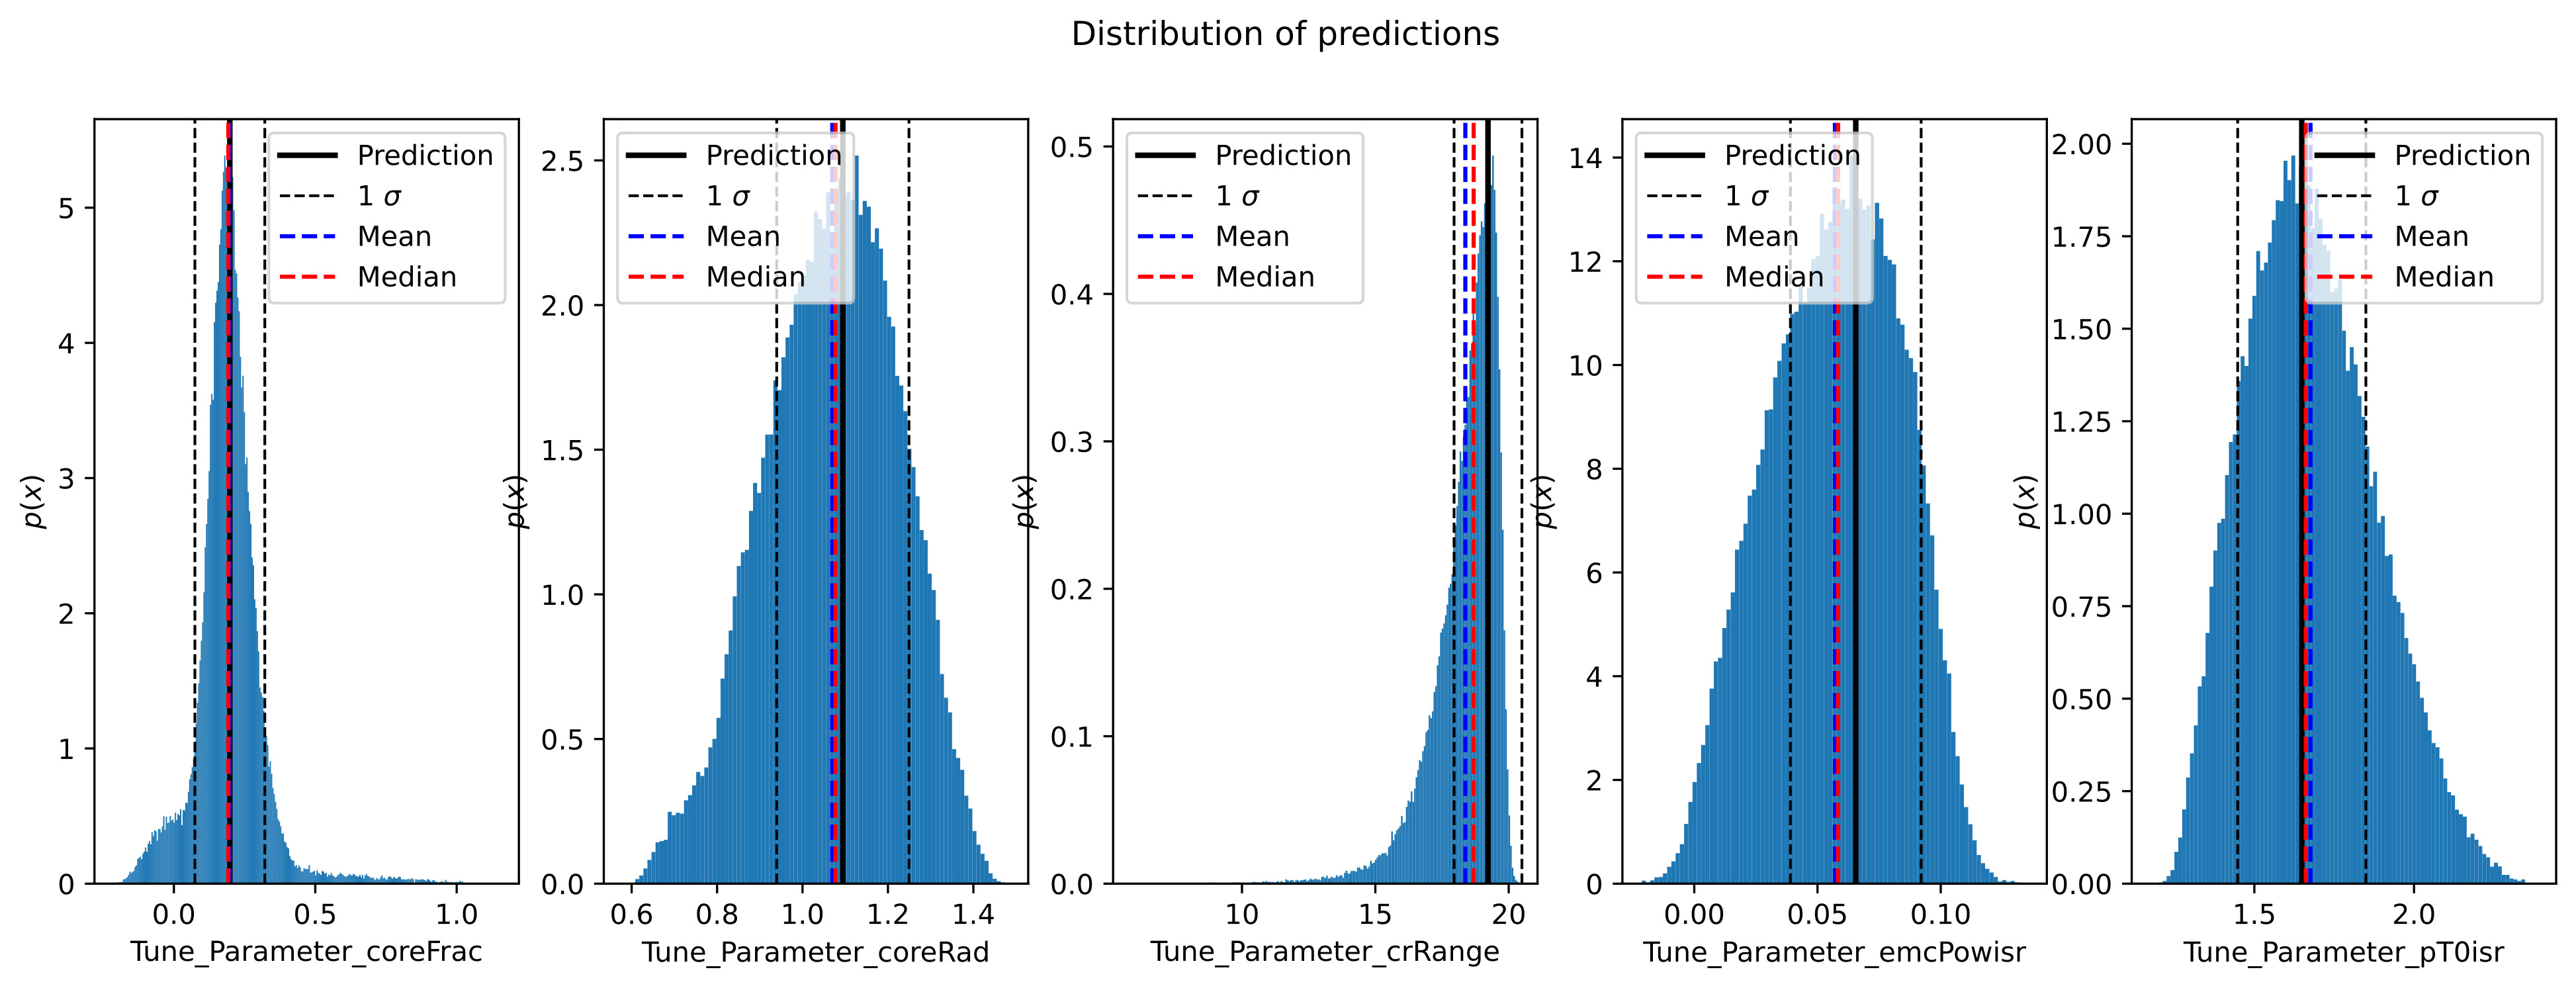
\includegraphics[width=0.9\textwidth]{{img/Plots_Totali_ext/prediction_spread.jpg}}
\caption{The spread of prediction obtained from the Inverse model. It is clear that also after the hyperparameters optimization the inverse model is not working properly. The distribution have long tails out of the limits for the variation, the central one refered to the Color Reconnection is predicted completely out of the boundaries.}
\label{fig:result_INV_5params}	
	\end{figure}

\begin{table}[!htb]
	\begin{tabular}{l | c | c}
		Parameter & Value & CP5 (down \& up)\\ \hline\hline
		\\[-0.85em]		
\texttt{MultipartonInteractions:pT0Ref} & $ 1.65 \pm 0.20  $ & $1.41 - 1.46$\\
\texttt{MultipartonInteractions:ecmPow} & $ 0.066 \pm 0.026 $ & $0.03$\\
\texttt{MultipartonInteractions:coreFraction} & $ 0.20 \pm 0.12 $ & $0.43 - 0.73$\\
\texttt{MultipartonInteractions:coreRadius} & $ 1.1 \pm 0.2 $ & $0.67 - 0.69$\\
\texttt{ColorReconnection:range} & $ 19.2 \pm 1.3 $ & $4.88 - 4.69$\\
\end{tabular}
\caption{The predicted values using Inverse model are showed here, the model is not working in this case the predicted values for the core radius and for the color reconnection are out of the boundary while other parameter are predicted with a quite large error.}
\label{table:result_INV_5params}
\end{table}

\noindent We can see from \figRef{fig:Inverse_not_working} the tune we get from the Inverse Model (blue line), as was expected, cannot describe the observables distributions.   The tune misses all the experimental data points approximately by a $50\%$ of the value. Se we have to exclude this model for this tune. Maybe the failure is related to the higher number of parameters respect to the first test, that leads to a more complex generator response and so a more difficult model to learn and invert.

In \textsc{mcnntunes} presentation paper \cite{MCNNTUNESarticle} is reported that the Inverse model can fail when in the training set is not given a sufficient number of MC simulations with parameters values near to the actual real ones. So, trying to make this model work, we decide to introduce a Gaussian bias in the sampling phase instead of a uniformed distributed sampling. Our Gaussian sampling was peaked on the parameters predicted by the PerBin Model, but also this procedure does not leads to some consistent results.   

\begin{figure}[H]
	\centering
	\noindent
	\begin{subfigure}{0.48\textwidth}
		\centering
		\includegraphics[width=\textwidth]{{img/Plots_Totali_ext/rivet-plots_5params/CMS_2015_PAS_FSQ_15_007/d01-x01-y01.pdf}}
	\end{subfigure}%
	\begin{subfigure}{0.48\textwidth}
		\centering
		\includegraphics[width=\textwidth]{{img/Plots_Totali_ext/rivet-plots_5params/CMS_2012_PAS_FSQ_12_020/d06-x01-y01.pdf}}
	\end{subfigure}%
	\caption{An example of the fact that the Inverse model (blue line) is not working: the bins are filled to only the $50\%$ of the expected value in almost all the bins. On the left is shown the transMIN charged particle transverse momentum sum density for the CMS analysis at $\sqrt{s}=13\ \mathrm{TeV}$ \cite{CMS-PAS-FSQ-15-007} and on the right the transMIN charged particle density from the CMS analysis \cite{CMS-PAS-FSQ-12-020} in both case as a function of the leading object transverse momentum.}
	\label{fig:Inverse_not_working}
\end{figure}


\subsection{Overall results}
\label{sec:result5params}

Overall, what we have are two tunes performed with the PerBin Model that are quite good tunes. In this section all the fitted distributions are shown and the two tunes are compared to the distribution obtained with the CP5 default values. The PerBin Model describe very well the data in particular in all the low-$p_T$ regions  where the experimental uncertainties are smaller and so more important in the $\chi^2$ evaluation.
\\
The first distributions showed in \figRef{fig:result_5params_1} are referred to the charged particle multiplicity and the charged particle scalar $p_T$ sum in the two transverse regions (TransMAX and TransMIN) as a function of the leading object transverse momentum. The black points are the experimental data taken from the CMS experiment at the center of mass energy of $13\ \mathrm{TeV}$. They are compared to the CP5 tune, red line, and the two tunes we have gotten from the PerBin Model and PerBin Model plus the re-weights, respectively blue and green lines. It is easy to see that all the three tunes are describing the distribution very well, in particular our tunes in the low-$p_T$ regions ($p_T<5 \ \mathrm{GeV}$) are describing the distribution also better than CP5 in most of the cases.

%%%% 13TEV
\begin{figure}[!htb]
	\centering
	\noindent
	\begin{subfigure}{0.48\textwidth}
		\centering
		\includegraphics[width=\textwidth]{{img/rivet-plots-MinBias_PerBin_vs_PerBinReweights_vs_CP5/CMS_2015_PAS_FSQ_15_007/d01-x01-y01.pdf}}
	\end{subfigure}%
	\begin{subfigure}{0.48\textwidth}
		\centering
		\includegraphics[width=\textwidth]{{img/rivet-plots-MinBias_PerBin_vs_PerBinReweights_vs_CP5/CMS_2015_PAS_FSQ_15_007/d02-x01-y01.pdf}}
	\end{subfigure}\\
	\begin{subfigure}{0.48\textwidth}
		\centering
		\includegraphics[width=\textwidth]{{img/rivet-plots-MinBias_PerBin_vs_PerBinReweights_vs_CP5/CMS_2015_PAS_FSQ_15_007/d05-x01-y01.pdf}}
	\end{subfigure}%
	\begin{subfigure}{0.48\textwidth}
		\centering
		\includegraphics[width=\textwidth]{{img/rivet-plots-MinBias_PerBin_vs_PerBinReweights_vs_CP5/CMS_2015_PAS_FSQ_15_007/d06-x01-y01.pdf}}
	\end{subfigure}
	\caption{In this figure the data from the $\sqrt{s}=13\ \mathrm{TeV}$ CMS analysis \cite{CMS-PAS-FSQ-15-007} that show the transMAX charged particle density (upper left) and the charged $p_T$-sum density (upper right); the transMIN charged particle density (lower left) and the charged $p_T$-sum density (lower right) as a function of the transverse momentum of the leading charged particle. The CP5 tune is compared to our tune using the PerBin Model. Our tune (red line) seems good as the CP5 (blue line) in describing the data. The first bins are the most important they have a smaller experimental error than the higher $p_T$  data. Also the PerBin model with re-weight (green line) seems really good in the description of the data. Also the ratio between MC and data points is reported and the green band represent the experimental uncertainties, while the  vertical colored lines on the MC points are the statistical uncertainties. }
	\label{fig:result_5params_1}
\end{figure}



\noindent Instead, in \figRef{fig:result_5params_2} are reported the same distribution but at $\sqrt{s}=7\ \mathrm{TeV}$ also in this case our tunes are good in describing the distributions, they seam to be also better than CP5.

%%%% 7TEV
\begin{figure}[!htb]
	\centering
	\noindent
	\begin{subfigure}{0.48\textwidth}
		\centering
		\includegraphics[width=\textwidth]{{img/rivet-plots-MinBias_PerBin_vs_PerBinReweights_vs_CP5/CMS_2012_PAS_FSQ_12_020/d05-x01-y01.pdf}}
	\end{subfigure}%
	\begin{subfigure}{0.48\textwidth}
		\centering
		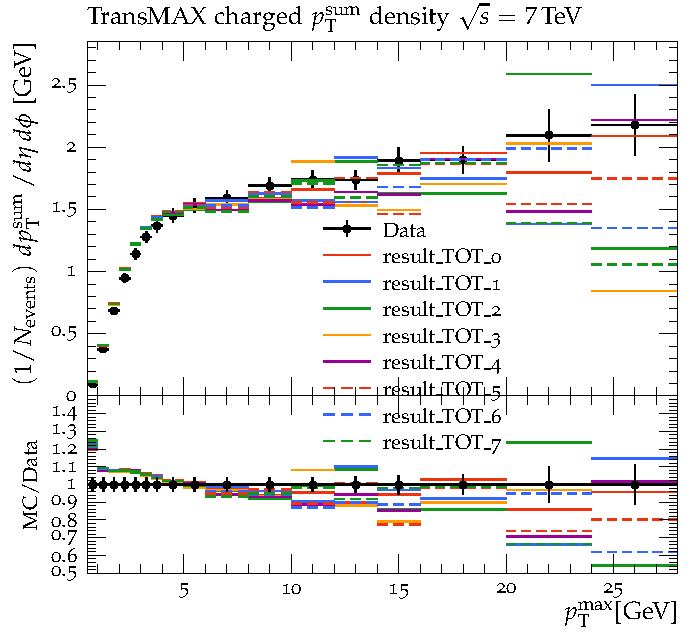
\includegraphics[width=\textwidth]{{img/rivet-plots-MinBias_PerBin_vs_PerBinReweights_vs_CP5/CMS_2012_PAS_FSQ_12_020/d08-x01-y01.pdf}}
	\end{subfigure}\\
	\begin{subfigure}{0.48\textwidth}
		\centering
		\includegraphics[width=\textwidth]{{img/rivet-plots-MinBias_PerBin_vs_PerBinReweights_vs_CP5/CMS_2012_PAS_FSQ_12_020/d06-x01-y01.pdf}}
	\end{subfigure}%
	\begin{subfigure}{0.48\textwidth}
		\centering
		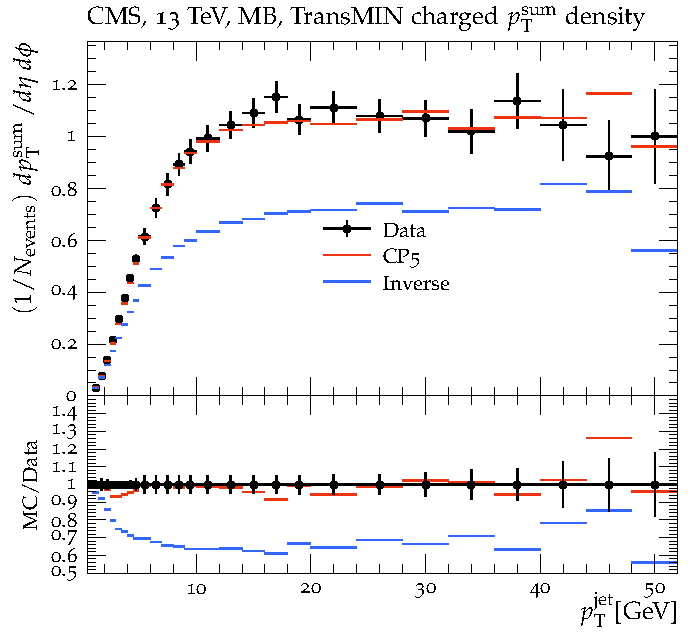
\includegraphics[width=\textwidth]{{img/rivet-plots-MinBias_PerBin_vs_PerBinReweights_vs_CP5/CMS_2012_PAS_FSQ_12_020/d09-x01-y01.pdf}}
	\end{subfigure}
	\caption{Here the data at $\sqrt{s}=7\ \mathrm{TeV}$ from the CMS analysis \cite{CMS-PAS-FSQ-12-020} for the transMAX charged particle density (upper left) and the charged $p_T$-sum (upper left); the transMIN charged particle density (lower left) and the charged $p-T$-sum are displayed as a function of the leading object transverse momentum. The three tunes describe the data (black point) very well. The low $p-T$ regions are described better from our tune respect to the CP5 tune. As was expected the result from the PerBin model with the re-weights (green line) are more similar to the CP5 result. Also the ratio between MC and experimental points is reported and the green band represent the experimental uncertainties, while the vertical colored lines on the MC points are the statistical uncertainties.}
	\label{fig:result_5params_2}
\end{figure}


\noindent Also the data at the center-of-mass energy of $1.96\ \mathrm{TeV}$ are well described. These data had been collected by the CDF experiment in proton-antiproton collisions.

%%%% 1.96TEV
\begin{figure}[!htb]
	\centering
	\noindent
	\begin{subfigure}{0.48\textwidth}
		\centering
		\includegraphics[width=\textwidth]{{img/rivet-plots-MinBias_PerBin_vs_PerBinReweights_vs_CP5/CDF_2015_I1388868/d01-x01-y01.pdf}}
	\end{subfigure}%
	\begin{subfigure}{0.48\textwidth}
		\centering
		\includegraphics[width=\textwidth]{{img/rivet-plots-MinBias_PerBin_vs_PerBinReweights_vs_CP5/CDF_2015_I1388868/d05-x01-y01.pdf}}
	\end{subfigure}\\
	\begin{subfigure}{0.48\textwidth}
		\centering
		\includegraphics[width=\textwidth]{{img/rivet-plots-MinBias_PerBin_vs_PerBinReweights_vs_CP5/CDF_2015_I1388868/d02-x01-y01.pdf}}
	\end{subfigure}%
	\begin{subfigure}{0.48\textwidth}
		\centering
		\includegraphics[width=\textwidth]{{img/rivet-plots-MinBias_PerBin_vs_PerBinReweights_vs_CP5/CDF_2015_I1388868/d06-x01-y01.pdf}}
	\end{subfigure}
	\caption{The transMAX charged particle density (upper left) and the charged $p_T$-sum (upper left); the transMIN charged particle density (lower left) and the charged $p_T$-sum from the CDF analysis at $\sqrt{s}=1.96\ \mathrm{TeV}$ in proton-antiproton collisions \cite{CDF:2015txs}. The data are described very well from the CP5, PerBin, PerBin + re-weights tunes. Also the ratio between MC and experimental points is reported and the green band represent the experimental uncertainties, while the vertical colored lines on the MC points are the statistical uncertainties.}
	\label{fig:result_5params_3}
\end{figure}

\noindent \figRef{fig:result_5params_4} and \figRef{fig:result_5params_5} represent the pseudorapidity distribution for diffractive events and for inelstaic charged hadrons production.
The left distribution of \figRef{fig:result_5params_4} and the distribution in \figRef{fig:result_5params_5} are not well described by the PerBin Model (blue line) but are better described by the PerBin Model plus the re-weights for these bins. So also in this case we have a good result from \textsc{mcnntunes} tool.

%%%% DIFFRACTIVE
\begin{figure}[!htb]
	\centering
	\noindent
	\begin{subfigure}{0.48\textwidth}
		\centering
		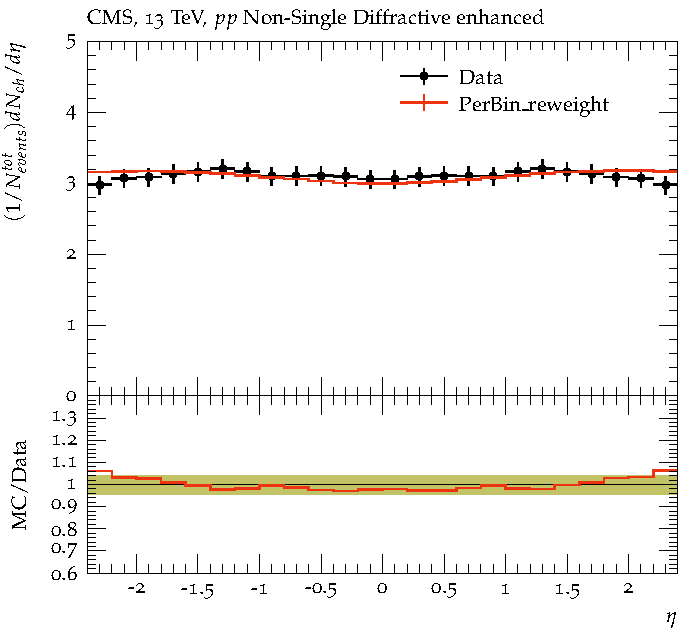
\includegraphics[width=\textwidth]{{img/rivet-plots-MinBias_PerBin_vs_PerBinReweights_vs_CP5/CMS_2018_I1680318/d01-x02-y01.pdf}}
	\end{subfigure}%
	\begin{subfigure}{0.48\textwidth}
		\centering
		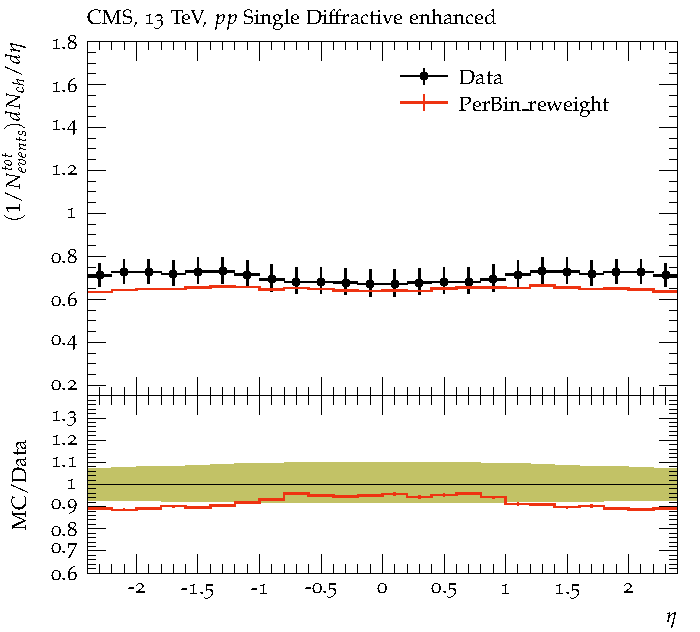
\includegraphics[width=\textwidth]{{img/rivet-plots-MinBias_PerBin_vs_PerBinReweights_vs_CP5/CMS_2018_I1680318/d01-x03-y01.pdf}}
	\end{subfigure}
	\caption{Here are reported the pseudorapidity distributions ($p_T > 0.5 \ \mathrm{GeV}$, $|\eta| < 2.4$) for charged particle multiplicity in single diffractive (right) and non-single diffractive (right) events selection. The black point are the data from the CMS analysis at $\sqrt{s}=13\ \mathrm{TeV}$ \cite{CMS:2018nhd}. The data from the \textsc{nsd} events are not so well described from the PerBin model (blue line) but with the re-weights we can describes these data points better. Instead, for the \textsc{sd} events we get a result equal to the one of CP5. Also the ratio between MC and data points is reported and the green band represent the experimental uncertainties, while the vertical colored lines on the MC points are the statistical uncertainties, in these distributions the statistical uncertainties are very small due to the high number of events in each bin.}
	\label{fig:result_5params_4}
\end{figure}

\begin{figure}[!htb]
	\centering
	\includegraphics[width=0.48\textwidth]{{img/rivet-plots-MinBias_PerBin_vs_PerBinReweights_vs_CP5/CMS_2015_I1384119/d01-x01-y01.pdf}}
	\caption{In this figure is shown the last distribution we use for the tune from the CMS analysis at $\sqrt{s}=13\ \mathrm{TeV}$ \cite{CMS:2015zrm}. The pseudorapidity distribution ($|\eta|<2$) for the charged hadron density in an inelastic proton-proton scattering selection. Also here the PerBin model (blue line) give a different result from the CP5 and the PerBin + re-weights tunes. Also the ratio between MC and data points is reported and the green band represent the experimental uncertainties, while the vertical colored lines on the MC points are the statistical uncertainties, in this distribution the statistical uncertainties are very small due to the high number of events in each bin.}
	\label{fig:result_5params_5}
\end{figure}

\medskip

A numerical evaluation on the overall difference between MC and experimental points can be evaluated for all the three tunes using the $\chi^2/\mathrm{DoF}$ definition:
\begin{equation}
	\chi^2=\displaystyle\sum_i\frac{(\text{MC}_i-\text{exp}_i)^2}{\sigma_i^2}\quad.
\end{equation}
The results we get are reported in \tableRef{table:chi2_MinBias}. 
\begin{table}[!htb]
	\centering
	\begin{tabular}{l  c }
		Tune & $\chi^2/\mathrm{DoF}$\\[2pt]\hline\hline
		\\[-0.85em]
		CP5: & 23.9\\[2pt]
		PerBin: & 13.7\\[2pt]
		PerBin + re-weights: & 19.4\\[2pt]
	\end{tabular}
	\caption{$\chi^2$ evaluation for the three tunes.}
	\label{table:chi2_MinBias}
\end{table}
From this is clear that from this evaluation the better tune overall is the PerBin model tune. In fact, the PerBin Model describes very well the distributions were the experimental uncertainties are smaller but don't describe very well the last distributions in the left panel of \figRef{fig:result_5params_4} and \figRef{fig:result_5params_5}. A very good result is also the one obtained from the PerBin Model with the different weights for the bins in the distribution in \figRef{fig:result_5params_5}. This tune in the idea of having a more general tune that describe better all the distributions can be considered as a better tune. In general the $\chi^2$ evaluated is less in both our tunes respect to the CP5 one. 
\\
Given these results we can conclude that \textsc{mcnntunes} is valid tool for the tune of the parameters in high energy physics generators. We obtained two valid tunes for the underlying event and minimum bias observations in proton-proton collisions.
\\
The activity observed in the two transverse regions and the pseudorapidity distributions for different events selections are well described after the tune of the parameters that control the multi parton interactions and the color reconnection in \textsc{pythia8}. 
\\
The output we got from the minimizer in \figRef{fig:minimization_5_params_PerBin} tell to us that the most important parameter for the description of this distributions is the threshold value $p_{T0}^{ref}$, all the distributions have a large sensitivity on the variation of this parameter and this is related to the well defined minimum we got.
\\ 
On the other hand the small dependence on the variation of the \texttt{Color}\-\texttt{Reconnection:}\-\texttt{range} parameter over a certain threshold indicate a saturation, in fact over some value almost all the possible color reconnection have taken place and so the model is less sensitive to this parameter.   
\\
The Inverse model instead in this case don't give us a good result but maybe further tests can take to some good results. Maybe increasing even more the training set size but with careful, \textsc{mcnntunes} does not present any control on the NNs typical over-fitting problem. Even if the Inverse Model don't give us a complete tune for the underlying events it perform very well in the first test. So, we cannot exclude it as a valid tool. 
\\
Now, that the tool is validated we are going to extend the tune procedure to some new distribution and parameter. In the next chapter we focus on the tune of the \textit{Primordial $k_T$} and Space Shower in order to improve the description of the data collected in $Z$ boson production events.




